\documentclass[a4paper,authoryear,review]{elsarticle}

\usepackage[utf8]{inputenc}
\usepackage{amssymb}
\usepackage{lineno}
\usepackage{url}
\usepackage{hyperref}
\usepackage{caption}
\usepackage{subcaption}
\usepackage{graphicx}
\usepackage{adjustbox}
\usepackage{epstopdf}
\usepackage{gensymb}
\usepackage{xcolor,colortbl}
% \usepackage[table,xcdraw]{xcolor}
% If you use beamer only pass "xcolor=table" option, i.e. \documentclass[xcolor=table]{beamer}
\usepackage[normalem]{ulem}
\useunder{\uline}{\ul}{}
%TODO: remover
\DeclareUnicodeCharacter{0301}{\'{e}}
\hypersetup{unicode=true,
           colorlinks=true,
           linkcolor=blue,
           citecolor=blue,
           filecolor=red,
           urlcolor=blue,
           breaklinks=true
           }

\journal{Journal of Computers and Electronics in Agriculture}

%% `Elsevier LaTeX' style
\bibliographystyle{elsarticle-harv}
%%%%%%%%%%%%%%%%%%%%%%%

\begin{document}

\begin{frontmatter}

\title{Deep Learning for 2D grapevine bud detection}

\author[utn]{Wenceslao Villegas Marset\corref{cor1}}
\ead{diego.villegas@alumnos.frm.utn.edu.ar}

\author[utn]{Diego Sebastián Pérez}
\ead{sebastian.perez@frm.utn.edu.ar}

\author[utn]{Carlos Ariel Diaz}
\ead{carlos.diaz@frm.utn.edu.ar}

\author[utn,conicet]{Facundo Bromberg}
\ead{fbromberg@frm.utn.edu.ar}

\address[utn]{Universidad Tecnológica Nacional, Facultad Regional Mendoza, Grupo de Inteligencia Artificial DHARMa, Dpto. de Sistemas de la Información. Rodríguez 273, CP 5500, Mendoza, Argentina.}

\address[conicet]{Consejo Nacional de Investigaciones Científicas y Técnicas (CONICET).}

\cortext[cor1]{Corresponding author}

\begin{abstract}
Visual inspection is a necessary task to measure relevant variables in viticulture susceptible to automation with computer vision methods. Bud detection is central for various of these tasks such as: measurement of bud sunlight exposure, autonomous pruning, bud counting, type-of-bud classification, bud geometric characterization, internode length, and bud development stage, among others. This paper presents a method for grapevine bud detection based on a \emph{Fully Convolutional Networks Mobile-Net} architecture. To validate its performance, this architecture was compared in the detection task with the known state-of-the-art method for bud detection, showing improvements over three aspects of detection: \emph{segmentation, correspondence identification} and \emph{localization}. In its best version of configuration parameters, the present approach showed a detection precision of $95.6\%$, a detection recall of $93.6\%$, a mean Dice coefficient of $89.1\%$ for correct detection (i.e., detections whose mask overlaps the true bud) with small and nearby false alarms (i.e., detections not overlapping the true bud) as shown by a mean pixel area of only $8\%$ the area of a true bud,  and a distance (between mass centers) of $1.1$ true bud diameters. The paper concludes with a discussion of the  advantages of our approach for real-world applications.
\end{abstract}

\begin{keyword}
Computer vision \sep Fully Convolutional Network \sep Grapevine bud detection \sep Precision viticulture
\end{keyword}
\end{frontmatter}

\linenumbers

%#######################################################################


\section{Introduction}

The present work proposes a solution for the autonomous detection of grapevine buds within 2D vineyard images captured in natural field conditions. The proposed approach is based on \emph{Fully Convolutional Networks} (FCN) \citep{long2015fully, shelhamer2017fully}, a sort of deep learning model specific for computer vision applications. The present solution contributes to the historical quest for more and better quality information about different vineyard processes that affect both the grapevine productivity and grape quality. 

For years, viticulturists have been producing models of the most relevant plant processes (i.e. fruit quality and yield, soil profiling, vine health) and have been gathering a wealth of information to feed into these models. Better and more efficient measuring procedures have resulted in more information, with its corresponding impact on the quality of model outcomes, while inspiring researchers to push the boundaries for producing more sophisticated models. Such information consists of a large set of variables for assessing different aspects of the plant parts involved in these processes: trunks, leaves, berries, buds, shoots, flowers, bunches, and canes. The list of variables is long, i.e.: berry maturity, number, weight, size and volume; cluster compactness, morphology, such as length, width, size, and elongation, as well as cluster volume, number and weight; bud burst, number and size; flower number, leaf area, shoot length, pruning weight, and canopy density, among others \citep{awriNDmanual1, awriNDmanual3}).

Nowadays, technology is pushing once again the possibilities regarding the quality and throughput of these measurements with improved digital and autonomous measurement procedures over manual ones. The discipline is experiencing a transition with many of its variables still being measured manually through visual inspection. This results in high labor costs that limit measurement campaigns to only small data samples which, even with the use of statistical inference or spatial interpolation techniques, limit outcome quality \citep{whelan1996spatial}. 

In some cases, this scenario is exacerbated by the need of experts for proper measurement, such as the case of variables associated with the plant phenological stages, such as bud swelling, bud burst, inflorescence, flowering, veraison, and berry ripening, among others \citep{lorenz1995growth}; or by a measurement procedure that requires the destruction of the plant part being measured, which prevents tracking a certain variable over time. Such is the case of the measurement of leaf area, bunch weight, berry weight and pruning weight \citep{kliewer2005leaf}. 

Precision viticulture in general \citep{bramley2009lessons}, and computer vision algorithms in particular, have been growing in the last couple of decades, mainly due to their potential for mitigating these limitations \citep{seng2018computer, matese2015technology}. These algorithms come along with the promise of an unprecedented boost in the production of vineyard information as well as many expectations not only about possible improvements in the quality of the model’s outcomes, but in its potential to produce better models by feeding all this information to big data algorithms. 

The present work contributes to this general endeavor with an algorithm for measuring variables related to one specific plant part: the bud, an organ of major importance as it is the growing point of the fruits, containing all the plant’s productive potential \citep{may2000bud}. Our contribution of autonomous bud detection not only enables the autonomous measurement of all bud-related variables currently measured by agronomists (see Table $\sim$\ref{tab:Tabla1} for a non-exhaustive list of bud-related variables), but it also has the potential to enable the measurement of novel, yet important, variables that at present cannot be measured manually. One example is the total sunlight captured by buds, which depends on the unfeasible manual task of determining the exact location of buds in 3D space.  Although the present work focuses on 2D detection, it could be easily upgraded to 3D by, for instance, integrating 2D detection into the workflow proposed by \citet{diaz2018grapevine} (c.f. Section $\sim$\ref{sec:related} for further details on this workflow).

Table $\sim$\ref{tab:Tabla1} shows a non-exhaustive list of the main bud-related variables currently measured by vineyard managers \citep{sanchez2005bud, noyce2016basis, collins2020effects}, together with an assessment of the extent to which detection contributes to their measurement. The right-most column indicates the information beyond detection necessary to complete the measurement, while the middle columns labeled (i), (ii), and (iii) indicate the specific aspects of detection required for that variable: (i) whether it requires a good  \emph{segmentation}, i.e., the discrimination of which pixels in the scene correspond to buds and which correspond to the background (non-bud); ii) a good \emph{correspondence identification}, i.e., discrimination of bud pixels as belonging to different buds; or (iii) a good \emph{localization}, i.e., the localization of the bud within the scene.

For instance, let us take the \emph{bud number} variable. On the one hand, If it is possible to correctly identify the matches, the bud number coincides directly with the detection count. On the other hand, for the \emph{type-of-bud classification}, in addition to identifying matches, the segmentation of the part of the image corresponding to the bud is necessary to feed a classifier with relevant visual information, minimizing the noise produced by background pixels. Lastly, to measure the \emph{incidence of sunlight on the bud}, segmentation is not necessary, but rather good bud localization, in addition to leaf 3D surface geometry.

\begin{table}[]
 \resizebox{\textwidth}{!}{%
\begin{tabular}{|l|c|c|c|l|}
\hline
Variable                                        & (i)     & (ii)     & (iii)     &                                   \\ \hline
Bud number                                  &     & x    &       & none                              \\ \hline
Bud area                                      & x       & x    &       & none                              \\ \hline
Type-of-bud classification                & x       & x    &       & plant structure (trunk and canes)     \\ \hline
Bud development stage               & x       & x    &       & classifier over bud mask        \\ \hline
Internode length (by bud detection)         &      & x       & x    & plant structure (trunk and canes)      \\ \hline
Bud volume                                    &      &      &       & 3D reconstruction            \\ \hline
Bud development monitoring         & x       & x    & x     &                                   \\ \hline
Incidence of sunlight on the bud          &      & x       & x    & 3D reconstruction, leaves 3D superficial geometry \\ \hline
\end{tabular}}
\caption{A non-exhaustive list of important bud-related variables accompanied by an assessment of the extent to which detection contributes to their measurement. The right-most column indicates the information beyond detection  necessary to complete the measurement, while the middle columns labeled (i), (ii), and (iii) indicate the three aspects of detection required: segmentation, correspondence identification, or localization, respectively.
}
\label{tab:Tabla1}
\end{table}

A good detector, therefore, should be evaluated on all three aspects of segmentation, correspondence identification and localization. This is easy for our detector as its implementation first produces a segmentation mask, which is then post-processed to produce correspondence identification and localization. The specific aspects of this approach are detailed in Section $\sim$\ref{sec:matmet}. The analysis of detection results presented in Section $\sim$\ref{sec:results} shows that this approach is superior to state-of-the-art algorithms for vine bud detection. Finally, Section $\sim$\ref{sec:discussion} discusses the scope, limitations of the results obtained for bud detection, sufficiency of the performance achieved for the measurement of a selection of variables in Table $\sim$\ref{tab:TablaXX}, as well as the most important conclusions, future work and potential improvements.

\subsection{Related work}
\label{sec:related}
A wide variety of research using computer vision and machine learning algorithms to acquire information about vineyards \citep{seng2018computer} can be found in the literature, such as berry and bunch detection \citep{nuske2011yield}, fruit size and weight estimation \citep{tardaguila2012automatic}, leaf area indices and yield estimation \citep{diago2012grapevine}, plant phenotyping \citep{herzog2014objective, herzog2014initial}, autonomous selective spraying \citep{berenstein2010grape}, and more \citep{tardaguila2012applications, whalley2013applications}. Among the outstanding computer algorithms in recent years, \emph{artificial neural networks} have aroused great interest in the industry as a means to carry out various visual recognition tasks \citep{hirano2006industry, kahng2017cti, tilgner2019multi}. In particular, \emph{Convolutional Neural Networks} (\textbf{CNNs}) have become the dominant machine learning approach to visual object recognition \citep{ning2017inception}. Two recent studies have successfully applied visual recognition techniques based on \emph{deep learning networks} to identify viticultural variables to estimate production in vineyards. One of them \citet{grimm2019adaptable} uses an FCN to carry out segmentation of grapevine plant organs such as young shoots, pedicels, flowers, buds or grapes. The other \citet{rudolph2018efficient} uses images of vines under field conditions that are segmented using a CNN to detect inflorescences, and over these segmented regions, the Circle Hough Transform algorithm is applied to detect flower buds.

Several works aim at detecting and locating buds in different types of crops by means of autonomous visual recognition systems. For instance, \citet{tarry2014integrated} presents an integrated system for chrysanthemum bud detection that can be used to automate labour intensive tasks in floriculture greenhouses. More recently, \citet{zhao2018research} presented a   computer  vision system used to  identify the  internodes and  buds  of  stalk  crops. To the best of our knowledge and research efforts, there are at least four works that specifically address the problem of bud detection in the grapevine by using autonomous visual recognition systems. The research work by \citet{xu2014detection}, \citet{herzog2014initial} and \citet{perez2017image} apply different techniques to perform 2D image detection involving different computer and machine learning algorithms. In addition, \citet{diaz2018grapevine} introduces a workflow to localize buds in 3D space. The most relevant details of each are presented below.

\citet{xu2014detection}’s study presents a bud detection algorithm using indoor captured RGB images and controlled lighting and background conditions specifically to establish a groundwork for an autonomous pruning system in winter. The authors apply a threshold filter to discriminate the background of the plant skeleton, resulting in a binary image. They assume that the shape of buds resembles corners and apply the \emph{Harris corner detector} algorithm over the binary image to detect them. This process obtains a recall of $0.702$, i.e., $70.2\%$ of the buds were detected. 

\citet{herzog2014initial}’s work presents three methods for bud detection, all of which are semi-automatic and require human intervention to validate the quality of the results. The best result is obtained using an RGB image with an artificial black background and corresponds to a recall of $94\%$. The authors argue that this recall is enough to solve the problem of phenotyping vines. They also argue that these good results can be explained by the particular green color and the morphology of the already sprouting buds of approximately $2cm$.  

\citet{perez2017image} outlines an approach for the classification of bud images in winter, using \emph{SVM} as a classifier and \emph{Bag of Features} to compute visual descriptors. They report a recall of over $90\%$ and an accuracy of $86\%$ when sorting images containing at least $60\%$ of a bud and a ratio of $20$-$80\%$ of bud vs. non-bud pixels. They argue that this classifier can be used in algorithms for 2D localization of the \emph{sliding windows} type due to its robustness to variation in window size and position. It is precisely this idea that has been reproduced in the present work to implement the baseline approach based on sliding windows and patch classifier.

Finally, \citet{diaz2018grapevine} introduces a workflow for the localization of buds in 3D space. The workflow consists of five steps. The first one reconstructs a 3D point cloud corresponding to the grapevine structure from several RGB images. The second step applies a 2D detection method using a sliding window technique and patch classification. The next step uses a voting scheme to classify each point in the cloud as a bud or non-bud. The fourth step applies the \emph{DBSCAN} clustering algorithm to group points in the cloud that correspond to a bud. Finally, in the fifth step, the localization is performed, obtaining the center of mass coordinates of each 3D point cluster. They report a recall of $45\%$ with an accuracy of $100\%$ and a localization error of approximately $1.5cm$, or 3 diameters of bud.  

Although these research studies represent a great advance in relation to the problem of detecting and localizing buds, they still show at least one of the following limitations (i) use of artificial background outdoors; (ii) controlled lighting indoors; (iii) need for user interaction; (iv) bud detection in very advanced stages of development; (v) low bud detection/classification recall, and (vi) although some of these works perform some kind of segmentation process as part of the approach, none of them aim to segment the bud or report metrics of the quality of the segmentation performed. These limitations represent a major barrier to the effective development of tools for measuring bud-related variables. 

\section{Materials and Methods}
\label{sec:matmet}

This section describes the main contribution of the present work, that is, the deep learning setup for 2D image detection of grapevine buds captured in natural conditions. Subsection $\sim$\ref{sec:fcn} provides details on the \emph{encoder-decoder} transfer learning architecture and the pre-training chosen for its encoder. 

The detection results achieved by this approach are contrasted with a bud detection method described in  \citet{perez2017image}. In this paper, the authors present a bud/non-bud image classifier and suggest its use for bud detection based on the idea of \emph{sliding windows}. Given an image of a viticultural scene, it subdivides it into a set of \emph{patches} or smaller regions \citep{perez2017image} and then detects buds by determining whether or not a certain patch contains a bud by using the image classifier. Our implementation of a detector based on this design is described in Subsection $\sim$\ref{sec:sw}. Finally, the section concludes with Subsection $\sim$\ref{sec:train} that provides details on the training of both methods including details on the  image collection used for its training. 

\subsection{Fully Convolutional Network with MobileNet (FCN-MN)}
\label{sec:fcn}

As outlined in the introduction, the approach proposes the use of computer vision algorithms to: (i) \emph{segment} buds by \emph{classifying} which pixels in the scene correspond to buds and which pixels correspond to background (non-buds), (ii) \emph{identify} bud \emph{correspondences} by discriminating those pixels that belong to different buds in the observed scene, and (iii) \emph{localize} each bud in the scene. 

For the segmentation operation, i.e., pixel classification, the fully convolutional network introduced in \citep{long2015fully} is taken as a basis and trained for the specific problem of grapevine bud segmentation. The following section  \ref{sec:fcnmn} describes in detail the architecture considered for these networks. The resulting fully convolutional network returns a probability map on the same scale as the original image, where the value of one pixel represents the probability that the corresponding pixel in the input image belongs to a bud. To obtain a binary mask, a classification threshold of $\tau$ is applied to each pixel, classifying the pixel as bud (non-bud) if its probability is higher (lower) than $\tau$. To identify bud correspondences, post-processing of this binary mask is performed to determine that two bud pixels correspond to the same bud, as long as they belong to the same connected component, i.e., joined by some sequence of contiguous bud pixels. 

Finally, there are several alternatives for the localization of objects among which are \emph{bounding box}, \emph{pixel-wise segmentation}, \emph{contour} and \emph{center of mass} of the \emph{object} \citep{lampert2008beyond}. In this work the last one was considered, choosing to localize buds by the center of mass of the connected component. 

\subsubsection {Encoder-decoder architecture}
\label{sec:fcnmn}

For the pixel classifier, the three versions -32s, 16s and 8s-  of the \emph{fully convolutional networks} originally introduced by \citet{long2015fully} were considered for their excellent results in many image segmentation applications \citep{litjens2017survey, garcia2018survey, kaymak2019brief}. These networks have characteristic architectures with two distinct parts: \emph{encoder} and \emph{decoder} (see $\sim$\ref{fig:FCN-MN}). 

The encoder consists of a convolutional neural network that performs a \emph{downsampling} of an input image into a feature set by means of convolution operations to produce a set of \emph{feature maps}, i.e., an abstract representation of the image that captures semantic and contextual information, but discards fine-grained spatial information. These operations reduce the spatial dimensions of the image as one goes deeper into the network, resulting in feature maps 1/n the size of the input image, where n is the downsampling factor. The decoder is an \emph{upsampling} subnet, which takes the low-resolution feature map set and projects it into pixel space, increasing the resolution to produce a segmentation mask (or dense pixel classification) with the same dimensions as the input image. This operation is implemented as a network of transposed convolutions with trainable parameters, also known as upsampling convolutions \citep{shelhamer2017fully}. 



\begin{figure}
    \centering
    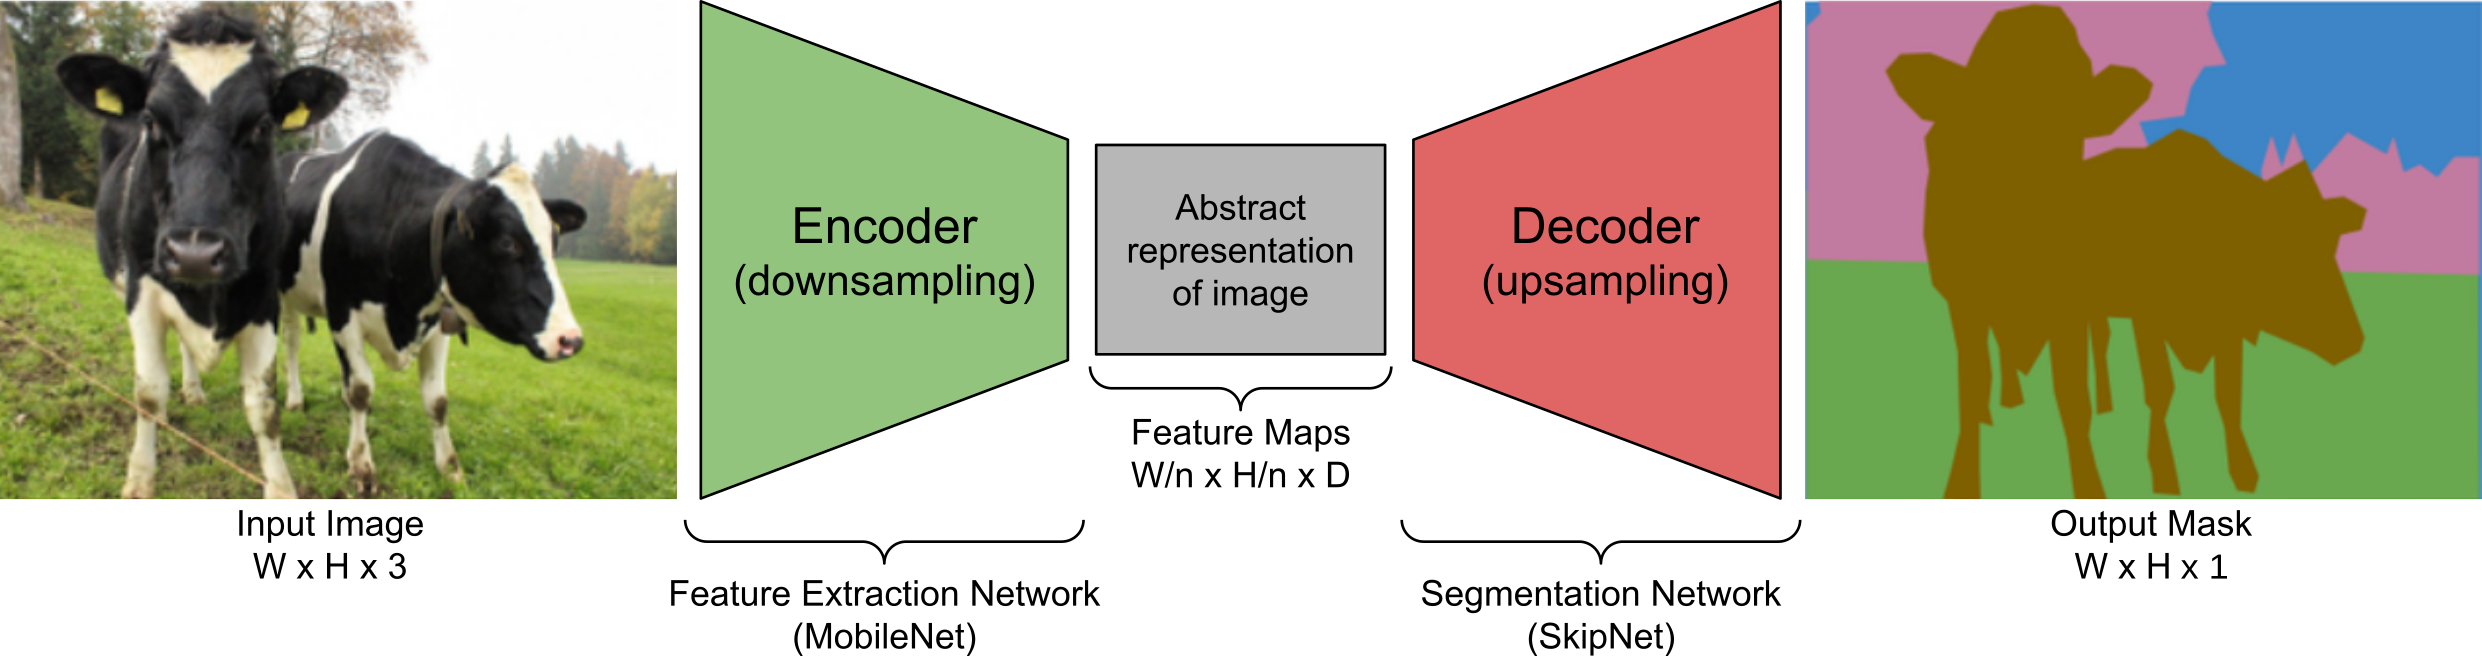
\includegraphics[width=12cm]{figures/Figure1.png}
    \caption{
Diagram of the FCN-MN network architecture proposed in this work, based on the FCN proposed by {shelhamer2017fully}, replacing its feature extraction encoder by MobileNet networks {howard2017mobilenets}, which produces feature maps with a $n$ downsampling factor. As a decoder for the production of the segmentation map, the SkipNet network {siam2018rtseg} is used implementing variants 32s, 16s and 8s.
    }
    \label{fig:FCN-MN}
\end{figure}

On the other hand, to refine segmentation quality, connections that go beyond at least one layer of the network, called \emph{skip connections}, are often used to transfer local spatial information from the internal encoder layers directly to the decoder. In general, these connections improve segmentation results, since they mitigate the loss of spatial information by allowing the decoder to incorporate information from internal feature maps, although their impact may vary depending on the proposed skip architecture. In \citet{long2015fully}, three skip architectures are proposed: 32s without information from internal encoder layers; 16s that adds spatial information from deep encoder layers; and 8s that adds spatial information from deep and less deep encoder layers. The details of these architectures are beyond the scope of this paper, but can be found in \citet{long2015fully} and \citet{shelhamer2017fully}. Since the results reported in the literature are not conclusive regarding which architecture is better,  \citet{long2015fully, shelhamer2017fully}, in this work all three alternatives are considered.

In spite of having achieved excellent results in practice, these architectures carry a significant load of computational resources. With this in mind, in this work the VGG encoder \citet{Simonyan2015VeryDC} originally proposed by Long for FCNs was replaced by the MobileNet network \citet{howard2017mobilenets}. This network stands out for its only $4.2$ million parameters against the 138 million VGG parameters, allowing the training and testing process to be considerably faster, with a much lower memory requirement, but maintaining performance. The use of MobileNet as an encoder in the fully convolutional networks of \citet{long2015fully} is not new, but had already been proposed for the 8s architecture by \citet{siam2018rtseg} in his SkipNet architecture. Technically, \citet{siam2018rtseg}’s proposal is extremely simple; that is why we dare extend it to the 16s and 32s architectures originally proposed by \citep{long2015fully}. It is due to these changes that for the rest of the paper these networks are referred to as \textbf{FCN-MN}.

\subsection{Sliding Windows detector}
\label{sec:sw}

This section describes the approach proposed by \citet{perez2017image} for the classification of bud images and its implementation for detection based on sliding windows described in the original paper. From now on, this detection approach will be referred to as SW. The approach follows three steps: (i) it applies the sliding windows algorithm to an image to extract patches (sub-images or rectangular regions); (ii) it sorts (all pixels of) each patch into bud or non-bud using the algorithm presented in \citet{perez2017image}; and (iii) it produces the final segmentation mask using a voting scheme. Details of each step are provided below.

Sliding windows techniques comprise a family of algorithms widely used in the past as part of various approaches to object localization with bounding boxes \citep{divvala2009empirical, wang2009hog, chum2007exemplar, ferrari2007groups, dalal2005histograms, rowley1996human}. In these algorithms, each image is scanned densely from one end of the image (e.g. upper left corner) to the other end (e.g. lower right corner) by a rectangular sliding window in different scales and different displacements, extracting sub-images or patches from the original image. In this work, 10 window sizes of equal height and width are defined, namely 100, 200, 300, 400, 500, 600, 700, 800, 900 and 1000 pixels, with a horizontal displacement of $50\%$ the width of the window and a vertical displacement of $50\%$ the height of the window, resulting in a $50\%$ overlap between contiguous patches. These values were chosen on the basis of the robustness analysis of the classifier presented by \citet{perez2017image} for the window geometry. This analysis shows that the classifier (explained in section \ref{sec:swtrain}) is robust for patches that contain at least $60\%$ of the pixels of a bud, and these must cover at least $20\%$ of the patch. If we consider extreme cases, i.e., the smallest bud diameter 100px and the largest 1600px, window sizes of 100px and 1000px could contain at least 60% of the pixels of a bud. In addition, using a 50% displacement, it is guaranteed that at least one patch will contain more than 20% bud pixels, 50px and 500px, respectively. The authors argue that a sliding window detection algorithm could easily propose a scheme for choosing window size and displacement to ensure that at some point in the scan the window meets robustness requirements. However, no details are given on how to implement it, so in this paper we only report results for fixed window sizes and explained displacement. Since the collection buds have a variable pixel diameter (corresponding to patches varying from 100×100 to 1600×1600 pixels, approximately), not all window sizes will be able to satisfy the robustness requirements for all patches, but the results can still be useful to make a comparison with the FCN-MN approach.  

The second step in this approach is to determine whether a patch is a bud or non-bud type. The classifier in  \citet{perez2017image} takes the patches produced by the sliding windows and, for each patch, it performs the following operations: (i) it computes low-level visual features using the \emph{Scale Invariant Feature Transform} (SIFT) \citet{lowe2004distinctive} algorithm; (ii) it builds a high-level descriptor for each patch using the \emph{Bag of Features} (BoF) \citet{csurka2004visual} algorithm on top of the SIFT features from the previous step; and (iii) it determines the class of each patch using the BoF descriptor on top of a classifier built using the \emph{Support Vectors Machine} \citet{vapnik2013nature} algorithm. Details of the training of this classifier are postponed until Section \ref{sec:swtrain} (SW training).

Finally, the third step of the approach is to build the binary mask where the pixels belonging to the bud and non-bud class are tagged. This mask is constructed through a voting scheme where each pixel adds one vote for each patch that contains it classified as a bud, which could be a maximum of four for some pixels, because the proposed displacement between patches has both horizontal and vertical overlap. Then, a minimum voting threshold of $\nu$ is established that can take values from 1 to 4, so that pixels with a number of votes equal to or greater than $\nu$ are classified as bud; otherwise, they are classified as non-bud. 

\subsection{Model training}
\label{sec:train}

This section provides details of the training process for each approach. In order to contrast both approaches they have been designed to receive the same type of input, i.e., an image of a viticultural scene, and to produce the same outputs, i.e., a binary mask of the same size as the original image whose positive pixels represent bud-type pixels, together with the  localization coordinates (X,Y) of these buds. This allows both to be trained with the same image collection, which is described in the following section, followed by model-specific training details.

\subsubsection{Image collection}
\label{sec:collection}

The image collection used in this study is the same collection originally used in \citet{perez2017image}, which has been downloaded from http://dharma.frm.utn.edu.ar/vise/bc as indicated by the authors. The complete collection consists of 760 images captured in winter in natural field conditions. However, in this work, only the 698 images containing exactly one bud were taken. Each image is accompanied by the ground truth, that is, a mask with manual segmentation of the bud. These images and their masks were used during the training and evaluation of the detection models. For this purpose, the image collection was separated into two disjoint subsets: the \emph{train set} with $80\%$ of the images and the \emph{test set} with the remaining  $20\%$. This resulted in a train set of 558 images and a test set of 140 images, both with their respective ground truth masks. In this way, the two proposed approaches use exactly the same 558 images during training and the same 140 images during testing.

\subsubsection{FCN-MN approach training}
\label{sec:fcntrain}

The 558 images reserved for this purpose were used to train this approach. These images have different resolutions; however, the three proposed FCN-MNs require a fixed size entry. Therefore, all images (including their masks) were scaled to a resolution of $1024 \times 1024$ pixels using a bilinear interpolation method \citep{han2013comparison}. In addition, for the train set images, the pixel RGB intensity values were scaled from [0.255] to [-1, 1].

Given the small number of images in the train set, two techniques widely used in practice were employed to achieve robust training: \emph{transfer learning} \citet{pan2009survey} and \emph{data augmentation} \citet{shorten2019survey}. The transfer learning process was carried out as follows: (i) the original  MobileNet network proposed by \citet{howard2017mobilenets} was implemented; (ii) the network was initialized with the parameters pre-trained on the ImageNet benchmark dataset \citet{kornblith2019better}; (iii) the MobileNet multi-class classification layer was replaced by a binary classification layer; (iv) the network was trained as a bud and non-bud patch classifier in an analogous way to SVM training, using the balanced patch train set after scaling all its images to $224 \times 224$ pixels; and (v) the parameters obtained in the previous step were used to initialize the encoder of our FCN-MN, introduced in Section \ref{sec:fcn}. The data augmentation process was applied on the fly during training, i.e., as the process required new images. For each train set image, 200 new images (111600 in total) were generated by simultaneously applying the following seven operations, whose values were taken at random with uniform probability: \emph{rotation} of up to $45\degree$; \emph{horizontal shifting} of up to $40\%$; \emph{vertical shifting} of up to $40\%$; \emph{shear} of up to $10\%$; \emph{Zoom} of up to $30\%$;  \emph{horizontal flip} and \emph{vertical flip}. 

For the training of the three  FCN-MN variants -8s, 16s, and 32s- it is required to specify the \emph{optimization method} and dropout value, two parameters typically defined by the user. In this work, the optimization methods considered were: \emph{Adam} with learning rate parameters= $0.001$, $beta1 = 0.9$ and $beta2 = 0.999$; \emph{RMSProp} with learning rate parameters = $0.001$ and $rho = 0.9$; and \emph{Stochastic Gradient Descent} with learning rate parameters = $0.0001$ and $momentum = 0.9$. For the dropout case, two values were considered: $0.5$ and $0.001$. These values were pre-selected by preliminary experiments not discussed here.

The best combination of optimization method and dropout was determined in training time over a validation set, using the \emph{4-fold cross validation} approach by 60 epochs and batchsize equal to $4$, varying over the three optimization methods and the two dropout values. The values selected were those that maximize the mean of Jaccard's \emph{Intersection-over-Union} (IoU) \citep{jaccard1912distribution}, a typical assessment measure in segmentation problems (see Section \ref{subsec:segmetrics}). For each combination of optimizer and dropout values the simple mean is reported between $12$ IoU corresponding to the $3$ variants considered in each of the $4$ folds. It can be observed in Table $\sim$\ref{tab:TablaX} that the combination of parameters with which the highest average IoU is reached is RMSProp with a dropout of $0.001$. 

\begin{table}[]
    \centering
    %\resizebox{0.5\textwidth}{!}
    \caption{
For each combination of optimizer and dropout values the simple mean is reported between $12$ IoU corresponding to the $3$ variants considered in each of the $4$ folds.
}
    \label{tab:TablaX}
\end{table}

Finally , the 3 variants were trained with RMSProp as an optimization method and a dropout value of $0.001$ over the complete training set for 200 epochs and batch size equal to 4.

\subsubsection{SW approach training}
\label{sec:swtrain}

The training stage for this approach is conducted in the same way as for the original workflow proposed in \citet{perez2017image}. This involves training a binary classifier to learn the concept of bud versus non-bud from a collection of rectangular patches that may or may not contain a bud. During the training, bud patches must be regions that perfectly circumscribe the bud while non-bud patches must be regions that do not contain a single bud pixel (see $\sim$\ref{fig:Figure2}). Therefore, to build the patch collection, the $558$ images and their masks were processed following the same protocol as in \citet{perez2017image}, obtaining a total of  $558$ patches circumscribing each bud (one per image) and more than $25000$ non-bud patches (the non-bud area is much larger than the area occupied by a bud in the image). The size of these patches is variable, with resolutions between $0.1$ and $2.6$ megapixels approximately (patches from $100 \times 100$ to $1600 \times 1600$ pixels).


\begin{figure}
    \centering
    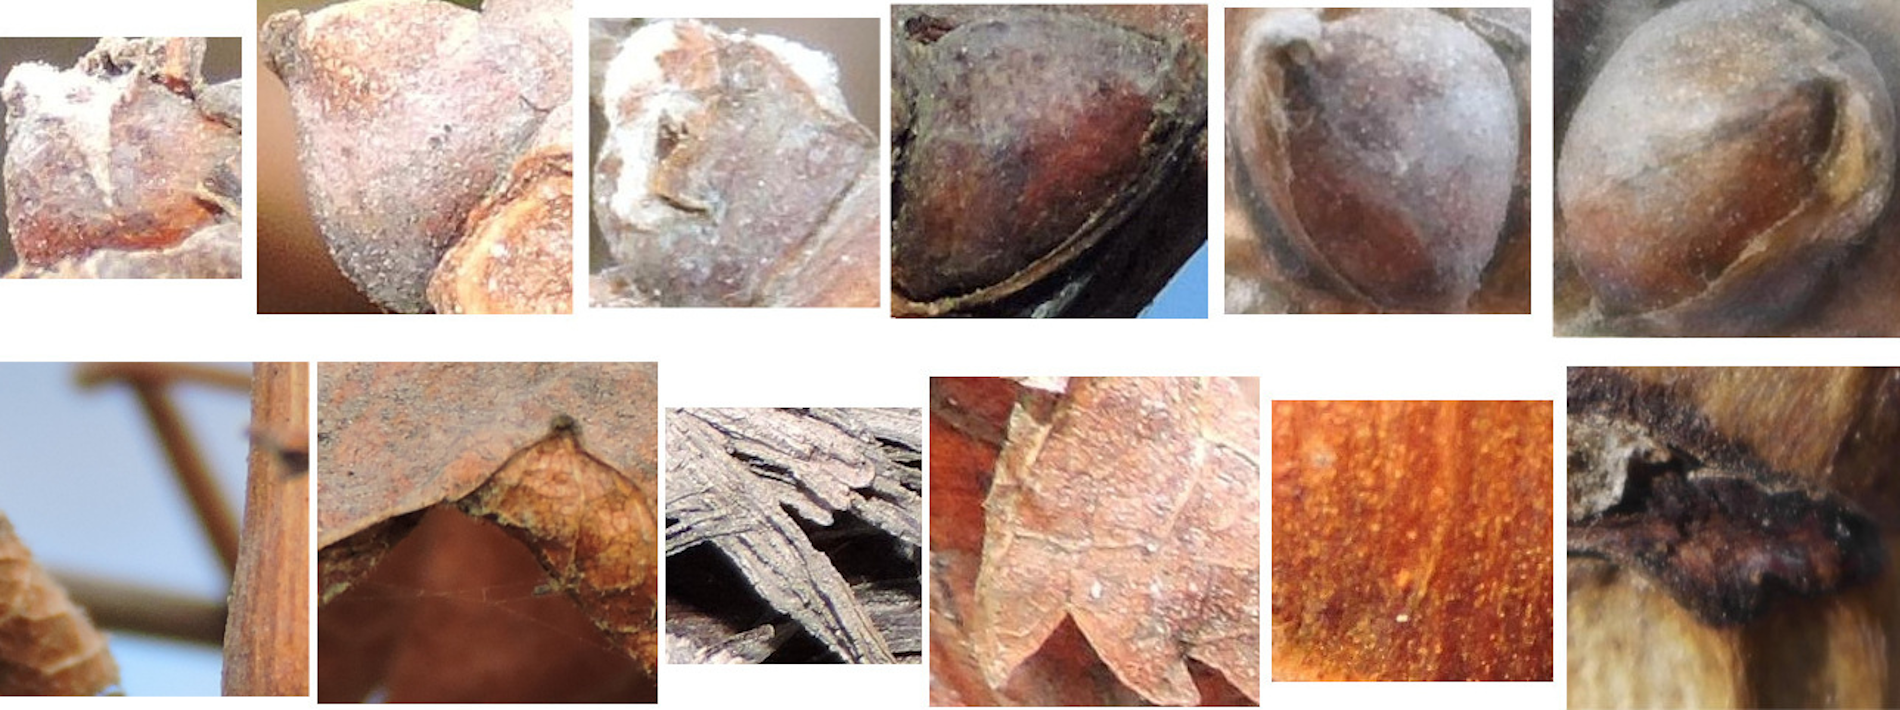
\includegraphics[width=12cm]{figures/Figure2.png}
    \caption{
Collection of patches used in this work. The first and second rows correspond to bud patches and non-bud patches, respectively. Image extracted from {perez2017image}.
    }
    \label{fig:Figure2}
\end{figure}


From this collection of patches, a balanced patch train set was created, i.e., with 558 patches of each class, where non-bud patches were taken at random from thousands of patches. The training was performed as detailed in the pipeline proposed by \citet{perez2017image}: (i) all SIFT descriptors were extracted from the train set; (ii) BoF was applied with a vocabulary size equal to 25, since it was the model with the best results according to the authors; and (iii) the SVM classifier was trained on the BoF descriptors of each patch using a \emph{Radial Basis Function} kernel, where the value of the $\gamma$ and $C$ parameters was established by means of a 5-fold cross-validation on the same value ranges, i.e., $\gamma = \{2^{-14}, 2^{-13}, \ldots, 2^{-7}\}$ and $C = \{2^{5}, 2^{6},\ldots , 2^{14}\}$.

\section{Experimental results} 
\label{sec:results}

In this section, a systematic evaluation of the quality of our proposed FCN-MN procedure for bud detection quality is presented. According to the discussion in the introduction, it can be decomposed into the three aspects that affect the relevant bud-related variables listed in Table $\sim$\ref{tab:TableX}: \emph{segmentation}, \emph{correspondence identification}, and \emph{localization}. 

For that purpose, the following subsection starts by presenting metrics that quantify the quality of these aspects, followed by the results in subsection $\sim$\ref{sec:results} that presents details on the metric values obtained for different experiments over the image test set. 

\subsection{Performance metrics}
\label{sec:metrics}

\subsubsection{Correspondence identification metrics}
\label{subsec:detectmetrics}

Correspondence identification of buds, both in  FCN-MN and SW, is the result of two steps: (i)  the thresholding of the algorithm’s output mask into a \emph{binary mask}, keeping all pixels of $\nu$ the probabilistic mask output by FCN-MN with values higher than $\tau$, and keeping all pixels that belong to at least $\nu$ patches rendered positive by SW, and (ii) the association of each \emph{connected component} of the binary mask to exactly one (detected) bud. 

Therefore, an incorrect correspondence identification is the result of an incorrect matching of detected components with actual buds in the image. This matching can become extremely complicated when there is an unknown number of true buds in the scene, as can be seen by the large amount of possible detection metrics defined in \citet{oguz2017dice}. To simplify the analysis, our image collection contains a single bud per image, avoiding the need for all the metrics that report the confusing situation of a component overlapping more than one true bud. This results in the following simplified list of possible metrics:

\begin{itemize}
\item \textbf{Correct Detection} ($CD$) is the best case and counts all images in the test collection for which the detected binary mask presents a single connected component, and this connected component overlaps with the true bud of the image. This would correspond with a \emph{true positive} situation.

\item \textbf{Split} ($S$) occurs when there is more than one detection per bud, which happens  when the mask contains multiple connected components, all of which overlaps the true bud. This metric counts the total number of images of the test collection whose detection is split.

\item \textbf{False Alarm} ($FA$) is equivalent to a \emph{false positive} situation and corresponds to connected components not overlapping the true bud. This measure counts the total number of such components over all images in the test collection.

\item \textbf{Detection Failure} ($DF$) is equivalent to a \emph{false negative} situation when the detection mask presents no connected components. It counts one for each image that satisfies this condition.
\end{itemize}

All four cases are mutually exclusive, that is, no image can satisfy any two (or more) of these definitions simultaneously. To quantify the correspondence identification quality, one could simply report these quantities counted over the test set, with the best case consisting in a $CD$ value equal to the cardinality of this set. However, determining the overall correspondence identification quality from the analysis of $4$ quantities can become rather complicated. 

One alternative is reporting the well-known precision and recall, denoted as $P_D$ and $R_D$, and referred to as \emph{detection-precision} and \emph{detection-recall} to distinguish them from the segmentation precision and recall defined further down. For that, the fact that there are two different true positive counts, $CD$ and $S$, needs to be addressed first. This is solved by first counting as true positives not only the $CD$ type of images, but also $S$, i.e., any image with either a correct detection or a split case is counted as one true positive, resulting in:

\begin{equation}
    P_D = \frac{true\ positives}{true\ positives+false\ positives} \\
= \frac{CD+S}{CD+S+FA}
    \label{eq:detection-precision}
\end{equation}

\begin{equation}
    R_D = \frac{true\ positives}{true\ positives+false\ negatives} \\
= \frac{CD+S}{CD+S+DF},
    \label{eq:detection-recall}
\end{equation}

and then account for the split type of errors by explicitly reporting $S$. 

Given these quantities, the \emph{F1-measure} computed as their harmonic average is also reported:
\[
    F1 = 2 \times \frac{precision \times recall}{precision + recall}.
\] 

\subsubsection{Segmentation metrics}
\label{subsec:segmetrics}

Correspondence identification metric, although informative, relies on the overlap between detected and true buds, regardless of how minimal the overlap is. This could miss several possible pixel-wise detection errors, resulting in rather coarse comparisons between competing detection algorithms. For instance, a correct detection could present a very small overlap with the true bud, with many or even a majority of the true bud pixels missing (i.e., several \emph{false negative} pixels), or it could be erroneously reporting several pixels as bud pixels (i.e., several \emph{false positive} pixels). Clearly, the best case scenario would be a case of correct detection with no false negative or positive pixels that would visually correspond to a perfect overlap between the detected connected component and the true bud. 

Similarly, a pixel-wise comparison of the masks could help assess split quality. The best split, for instance, would be one completely enclosed within the true mask -i.e., with none of its connected components presenting false positive pixels-, while covering as much of the true bud mask as possible, i.e., presenting just enough false negatives to disconnect its components. Finally, a false alarm case, clearly presenting only false positive pixels, could be further assessed by the number of (false positive) pixels in its components. 

The community has proposed several metrics to quantify segmentation errors. The most obvious ones are those that report the \emph{fraction} of the whole image corresponding to \emph{true positive} pixels, denoted as $TPF$; \emph{false positive} pixels,  denoted as $FPF$;  and \emph{false negative} pixels, denoted as $FNF$. As for the correspondence identification metric, one can simplify the analysis by considering pixel-wise precision and recall, denoted as  $P_S$ and $R_S$ and referred to as \emph{segmentation precision} and \emph{segmentation recall}, defined formally as: 

\begin{eqnarray*} 
    P_S &=& TPF / (TPF + FPF) \\
    R_S &=& TPF / (TPF + FNF),
\end{eqnarray*}

accompanied by their weighted harmonic mean, the well-known \emph{F-measure}, 

\begin{equation} 
   2 \times precision \times recall / (precision + recall),
\end{equation}

proposed independently by \citet{dice1945measures}; thus, usually referred to as the \emph{Dice measure}. A common alternative to the Dice measure is Jaccard’s \emph{intersection-over-union} \citep{jaccard1912distribution} equivalent to $TPF / (TPF+FPF+FNF)$. 

With these metrics, one could quantify the refinements discussed in the first paragraph above by simply applying them, not to the whole mask, but to the individual correspondence identification cases; for instance, by reporting the mean Dice measured over all correctly detected components. Or else, by refining the assessment of how bad a split is, one could report the mean Dice measure to all components of some split or the mean Dice measure over all split components of all split images. 

The case of false alarms is rather monotonous and not very informative with zero precision and recall for all such components. Indeed, a pixel-wise assessment of the gravity of a false alarm requires a quantification of the number of false positive pixels. One could simply consider the $FPF$, the fraction of all the false positive image pixels. Instead, we considered a normalization against bud size to be more informative, resulting in the \emph{normalized area}, denoted as $NA$ and defined formally as \emph{the total area of the component corresponding to its total number of pixels normalized by the area of the true bud}. 

\subsubsection{Localization metrics}
\label{subsec:locmetrics}

As a localization metric we propose the \emph{normalized distance}, denoted as $ND$, defined formally as \emph{the distance between the center of mass of the component and the center of mass of the true bud, divided by the diameter of the true bud (defined as the maximum distance between any two border points of the true bud)}.

\subsection{Results}
\label{sec:resultados}

We shall proceed now to assess the validity of our main hypothesis, namely, that FCN-MN is a better detector than its SW counterpart over each of the metrics defined in the previous section. 

For a thorough comparison, several cases for each algorithm  were considered: training $27$ FCN-MN detectors and $40$ SW detectors over the training set of $558$ images, one for each combination of their respective hyper-parameters. For FCN-MN, these hyper-parameters are the three architectures -8s, 16s, and 32s- and the $9$ values $\{0.1, 0.2, \ldots, 0.9\}$ for the binarization threshold $\tau$. For SW, in turn, these hyper-parameters are the $10$ patch sizes $\{100, 200, \ldots, 1000\}$  and the $4$ values $\{1, 2, 3, 4\}$  of the voting threshold $\nu$.

Table $\sim$\ref{tab:TablaXX} shows the results for the best detectors of each algorithm, reporting all performance metrics of the three aspects of detection: correspondence identification, segmentation and localization. The first column shows the label of the selected detectors, with the subscript indicating the architecture and patch size for the case of FCN-MN and SW, respectively, and the superscript indicating the thresholds $\tau$ and $\nu$, respectively.

The table includes all metrics defined in Section $\sim$\ref{sec:metrics} required for a thorough comparison of FCN-MN against SW. First, four correspondence identification metrics are included: detection precision $P_D$, detection recall $R_D$, the F1-measure  $F1$, and $S$ (the total count of split components). 

For a thorough analysis of the segmentations, the segmentation metrics for the correct detections, splits and false alarms were differentiated. For the detections -i.e., correct detections and splits-, we report segmentation precision, segmentation recall, and the Dice measure denoted in the table by $P_S^{CD}$, $R_S^{CD}$ and $Dice^{CD}$ for correct detections and $P_S^S$, $R_S^S$ and $Dice^S$ for splits.  Each of the three correctly detected cells report the mean value of the measure computed for each correctly detected test image, i.e., each image with only one component overlapping the true bud, including the corresponding standard deviation  in parenthesis. For the split group, the mean and standard deviation are computed over the measures computed only for the split images, i.e., over the images containing at least two components overlapping the true bud. Here, the segmentation metrics are computed over the union of all split components. 

For the false alarms, the mean \emph{normalized area} ($NA$) is reported, in this case computed individually for each false alarm component, reporting at each cell its mean over all false alarm components of all test images. Finally, for localization, the table reports the \emph{normalized distance} ($ND$), but \emph{only} the mean and standard deviation (in parenthesis) over all false alarms components. As they overlap the true bud, correctly detected and splitted components should be so close to the true bud that no major analysis should be necessary. But for the sake of completeness,  some statistics are included below. 
%

The table is a summary, as it includes only a subset of all $27$ FCN-MN cases and a subset of all $40$ SW cases. A detector was considered for inclusion in the table if, when compared to its counterparts of the same algorithm, it resulted in the highest value for at least one of the metrics. The corresponding cell was marked in bold in the table. For instance, the detector FCN-MN$_{16s}^{0.8}$ has been included because its detection precision $P_D$ of $97.7$ is the largest among the detection precision of all $27$ FCN-MN detectors. Similarly, the detector SW$_{1000}^1$ has been included because its precision $P_D = 67.0$ is the largest among all $40$ SW detectors. 

The table shows a clear improvement of FCN-MN over SW. For all metrics, the best  FCN-MN detector (bolded) improves (or ties) over the best SW detector (bolded) represented in the table by underlying the detector with the best metric. The exception is the two segmentation recalls (for correct detections and splits) for which the SW case has a better (larger) mean, $98.8$ versus $99.9$ for correct detections and $74.7$ versus $78.6$ for the split case; and the total split count $S$, with the best case for FCN-MN being $1$ and $0$ for the best SW case. These improvements are not statistically significant, however, due to the large standard deviations of the FCN-MN cases, of $3.4$ and $8.1$ for correct detections and splits, respectively,  resulting in (statistically) overlapping values. 

In some cases, the improvements of FCN-MN over SW are overwhelming. For instance, for detection-precision, correctly detected segmentation-precision, and split segmentation-precision, the FCN-MN over SW improvements are $97.7$ versus $67.0$, $98.1$ versus $46.5$, and $99.9$ versus $67.5$, respectively.  In addition, for the $NA$ and $ND$ of false alarms, the  FCN-MN versus SW improvements are $0.04$ versus $0.22$ and $1.1$ versus $6.0$, respectively. 










\begin{table}[]
    \scriptsize
    %\tiny
    \centering        
    \begin{adjustbox}{angle=90}
        \resizebox{.90\textheight}{!}{%
           \begin{tabular}{lcccccccccccc}
                \hline
                \multicolumn{1}{|l|}{\textbf{Detector}} & \multicolumn{1}{c|}{\textbf{$P_D$}} & \multicolumn{1}{c|}{\textbf{$R_D$}} & \multicolumn{1}{c|}{\textbf{$F1$}} & \multicolumn{1}{c|}{\textbf{$S$}} & \multicolumn{1}{c|}{\textbf{$P_S^{CD}$}} & \multicolumn{1}{c|}{\textbf{$R_S^{CD}$}} & \multicolumn{1}{c|}{\textbf{$Dice^{CD}$}} & \multicolumn{1}{c|}{\textbf{$P_S^S$}} & \multicolumn{1}{c|}{\textbf{$R_S^S$}} & \multicolumn{1}{c|}{\textbf{$Dice^S$}} & \multicolumn{1}{c|}{\textbf{$NA$}} & \multicolumn{1}{c|}{\textbf{$ND$}} \\ \hline
                FCN-MN$_{8s}^{0.5}$ & 75.4 & 98.6 & 85.4 & 2 & 91.0 (11.3) & 90.2 (11.7) & {\ul \textbf{89.6 (10.3)}} & 96.6 (2.2) & 73.1 (17.6) & {\ul \textbf{82.1 (10.2)}} & 0.26 (0.69) & 3.72 (4.64) \\
                FCN-MN$_{8s}^{0.9}$ & 90.1 & 97.1 & 93.5 & 8 & {\ul \textbf{98.1 (6.0)}} & 68.3 (21.1) & 77.9 (19.6) & 98.7 (3.0) & 57.4 (18.4) & 70.8 (13.6) & 0.24 (0.5) & 3.8 (5.66) \\
                FCN-MN$_{16s}^{0.1}$ & 71.3 & {\ul \textbf{100}} & 83.2 & 6 & 75.7 (13.1) & 95.4 (14.7) & 83.1 (13.5) & 83.1 (8.9) & 54.1 (21.9) & 61.9 (17.5) & 0.12 (0.44) & 5.27 (6.53) \\
                FCN-MN$_{16s}^{0.4}$ & 87.0 & 96.4 & 91.5 & \textbf{1} & 87.7 (12.1) & 89.8 (18.2) & 87.0 (15.6) & 96.7 (0.0) & 37.0 (0.0) & 53.5 (0.0) & {\ul \textbf{0.04 (0.09)}} & 3.8 (5.08) \\
                FCN-MN$_{16s}^{0.6}$ & 95.6 & 93.6 & 94.6 & 3 & 92.2 (8.7) & 88.2 (13.3) & 89.1 (10.7) & 99.4 (0.6) & 16.2 (10.6) & 26.6 (16.8) & 0.08 (0.11) & {\ul \textbf{1.1 (0.65)}} \\
                FCN-MN$_{16s}^{0.8}$ & {\ul \textbf{97.7}} & 92.1 & {\ul \textbf{94.9}} & 4 & 95.8 (7.0) & 81.6 (14.6) & 87.0 (10.7) & 99.7 (0.3) & 34.2 (32.6) & 43.9 (33.1) & 0.1 (0.12) & 1.28 (0.95) \\
                FCN-MN$_{16s}^{0.9}$ & {\ul \textbf{97.7}} & 91.4 & 94.5 & 4 & 97.6 (5.6) & 74.5 (16.5) & 83.1 (12.8) & {\ul \textbf{99.9 (0.1)}} & 31.8 (27.9) & 41.6 (34.0) & 0.07 (0.11) & 1.33 (0.9) \\
                FCN-MN$_{32s}^{0.1}$ & 35.4 & {\ul \textbf{100}} & 52.2 & 8 & 67.4 (14.0) & \textbf{98.8 (3.4)} & 79.1 (11.0) & 86.0 (9.4) & 73.4 (19.6) & 77.1 (10.4) & 0.14 (0.66) & 4.62 (5.59) \\
                FCN-MN$_{32s}^{0.2}$ & 50.9 & {\ul \textbf{100}} & 67.5 & 10 & 73.9 (13.6) & 98.1 (3.8) & 83.5 (10.1) & 92.2 (5.4) & 53.4 (25.8) & 63.6 (19.3) & 0.17 (0.55) & 4.33 (6.17) \\
                FCN-MN$_{32s}^{0.3}$ & 49.8 & {\ul \textbf{100}} & 66.5 & 10 & 79.1 (13.2) & 95.5 (10.5) & 85.2 (11.8) & 88.5 (9.7) & 61.0 (35.1) & 65.8 (28.2) & 0.1 (0.39) & 3.68 (5.62) \\
                FCN-MN$_{32s}^{0.6}$ & 68.5 & 99.3 & 81.1 & 16 & 89.0 (11.5) & 89.1 (11.3) & 88.1 (9.6) & 92.4 (7.7) & \textbf{74.7 (28.1)} & 78.1 (24.0) & 0.11 (0.3) & 2.95 (4.36) \\
                SW$_{100}^{1}$ & 9.4 & {\ul \textbf{100}} & \textbf{17.2} & 28 & 24.6 (17.7) & 86.7 (19.5) & 33.6 (15.1) & 57.9 (28.2) & 24.8 (16.8) & 27.9 (13.8) & 1.08 (3.2) & 7.68 (6.02) \\
                SW$_{100}^{3}$ & 14.6 & 93.1 & 25.3 & 40 & 42.4 (26.4) & 56.8 (29.9) & \textbf{39.9 (19.7)} & 55.5 (32.2) & 24.8 (18.1) & 26.0 (15.6) & 0.31 (0.96) & 6.45 (6.19) \\
                SW$_{100}^{4}$ & 19.5 & 87.4 & 31.9 & 49 & \textbf{46.5 (29.3)} & 39.2 (28.9) & 33.9 (21.1) & 49.0 (29.0) & 20.1 (13.7) & 24.1 (14.0) & \textbf{0.22 (0.57)} & \textbf{6.0 (6.56)} \\
                SW$_{200}^{1}$ & 20.0 & {\ul \textbf{100}} & 33.3 & 12 & 16.6 (12.5) & 94.9 (13.5) & 25.9 (14.2) & 49.3 (26.4) & 40.2 (17.4) & 36.8 (11.9) & 5.13 (19.3) & 7.56 (5.35) \\
                SW$_{200}^{3}$ & 26.0 & 98.6 & 41.1 & 19 & 29.9 (17.0) & 74.7 (27.3) & 38.5 (17.0) & \textbf{67.5 (32.7)} & 16.5 (8.9) & 24.2 (11.9) & 1.69 (3.15) & 8.94 (6.22) \\
                SW$_{300}^{1}$ & 26.9 & {\ul \textbf{100}} & 42.4 & 2 & 13.7 (13.6) & 97.0 (9.6) & 21.6 (15.5) & 55.0 (11.8) & 48.1 (1.1) & \textbf{50.8 (4.5)} & 7.79 (20.5) & 6.83 (4.44) \\
                SW$_{400}^{1}$ & 32.7 & {\ul \textbf{100}} & 49.3 & 2 & 10.5 (11.7) & 98.7 (9.3) & 17.2 (15.3) & 42.6 (10.1) & 61.9 (11.6) & 50.4 (10.9) & 11.59 (24.05) & 7.12 (4.15) \\
                SW$_{400}^{2}$ & 34.6 & {\ul \textbf{100}} & 51.4 & 4 & 15.6 (15.1) & 94.5 (13.3) & 23.8 (15.6) & 48.7 (27.6) & 36.0 (4.6) & 38.6 (13.1) & 9.54 (26.13) & 7.88 (4.89) \\
                SW$_{500}^{1}$ & 40.2 & {\ul \textbf{100}} & 57.3 & 1 & 8.40 (9.7) & {\ul \textbf{99.9 (4.9)}} & 14.2 (13.8) & 17.9 (0.0) & {\ul \textbf{78.6 (0.0)}} & 29.2 (0.0) & 17.39 (30.07) & 7.22 (4.04) \\
                SW$_{500}^{2}$ & 38.6 & {\ul \textbf{100}} & 55.7 & 1 & 13.5 (14.0) & 95.2 (14.5) & 21.0 (16.0) & 35.2 (0.0) & 45.9 (0.0) & 39.8 (0.0) & 17.19 (39.07) & 7.56 (4.42) \\
                SW$_{600}^{1}$ & 43.5 & {\ul \textbf{100}} & 60.6 & {\ul \textbf{0}} & 6.9 (7.8) & 98.5 (10.7) & 12.0 (12.0) & nan (nan) & nan (nan) & nan (nan) & 25.48 (48.45) & 7.72 (4.3) \\
                SW$_{600}^{2}$ & 41.7 & {\ul \textbf{100}} & 58.8 & 1 & 10.4 (10.6) & 93.7 (18.9) & 17.2 (14.4) & 19.7 (0.0) & 27.2 (0.0) & 22.9 (0.0) & 20.41 (38.32) & 7.92 (4.38) \\
                SW$_{700}^{1}$ & 50.6 & {\ul \textbf{100}} & 67.2 & {\ul \textbf{0}} & 5.6 (6.5) & 98.6 (12.0) & 9.9 (10.3) & nan (nan) & nan (nan) & nan (nan) & 31.95 (64.36) & 7.75 (4.45) \\
                SW$_{800}^{1}$ & 56.7 & {\ul \textbf{100}} & 72.4 & {\ul \textbf{0}} & 5.1 (6.6) & 97.7 (11.0) & 9.0 (10.4) & nan (nan) & nan (nan) & nan (nan) & 44.53 (71.52) & 7.7 (4.06) \\
                SW$_{800}^{2}$ & 49.6 & 99.2 & 66.1 & {\ul \textbf{0}} & 8.3 (9.4) & 95.0 (15.9) & 13.9 (13.2) & nan (nan) & nan (nan) & nan (nan) & 30.52 (46.45) & 7.82 (4.1) \\
                SW$_{900}^{1}$ & 64.3 & {\ul \textbf{100}} & 78.3 & {\ul \textbf{0}} & 4.2 (5.7) & 94.7 (19.0) & 7.5 (9.2) & nan (nan) & nan (nan) & nan (nan) & 48.16 (80.31) & 7.9 (4.35) \\
                SW$_{900}^{3}$ & 42.2 & 92.4 & 58.0 & {\ul \textbf{0}} & 15.0 (14.8) & 81.5 (28.9) & 22.7 (16.8) & nan (nan) & nan (nan) & nan (nan) & 17.97 (29.56) & 7.65 (4.67) \\
                SW$_{1000}^{1}$ & \textbf{67.0} & {\ul \textbf{100}} & \textbf{80.2} & {\ul \textbf{0}} & 3.7 (4.7) & 95.3 (18.3) & 6.8 (7.9) & nan (nan) & nan (nan) & nan (nan) & 57.83 (84.87) & 7.91 (4.3) \\
                SW$_{1000}^{2}$ & 56.7 & 98.3 & 71.9 & {\ul \textbf{0}} & 6.3 (6.9) & 93.8 (19.1) & 11.1 (10.9) & nan (nan) & nan (nan) & nan (nan) & 47.26 (68.92) & 7.98 (4.44) \\ \hline
            \end{tabular}     
        }
    \end{adjustbox}
     \caption{
Correspondence identification, segmentation and localization metrics for the best FCN-MN and SW detection models.   Each column shows two bolded cells corresponding to the cell with the best metric among all FCN-MN rows and the cell with best metric among SW rows. The larger of the two has been underlined, representing the best among all combined models, i.e., the best of the column.  Columns $P_D$, $R_D$, $F1$ and $S$ show results for the \emph{Correspondence identification metrics} detection precision, detection recall, F1-measure and number of images with splits, respectively: Columns $P_S^{CD}$, $R_S^{CD}$ and $Dice^{CD}$ (resp. $P_S^S$, $R_S^S$ and $Dice^S$) correspond to the \emph{segmentation metrics} mean segmentation precision, mean segmentation recall, and mean Dice measure over all correctly detected components (resp. split components); and Columns $NA$ and $ND$ show the mean $NA$ and mean $ND$ over all false alarm components.
    }
        \label{tab:TablaXX}
\end{table}


\subsubsection{Detailed analysis of correspondence identification metrics}
\label{sub:compFCNSW}

Graphically, one could expect a better combined analysis of detection-precision and detection-recall than could be obtained by comparing the F1-measure. This is shown as a scatter plot in Figure $\sim$\ref{fig:detection-scatter-plot}, a graphical representation of a non-summarized version of the second and third columns of Table $\sim$\ref{tab:TablaXX}. Each dot  in the plot is located according to the detection-precision and detection-recall, and the color black or white, whether it corresponds to an FCN-MN or an SW detection model.

The graph reinforces the clear and undisputed improvements of FCN-MN over SW already detected in the table, with similar detection-recalls, but larger detection-precisions over most scenarios. 


 \begin{figure}
    \centering
    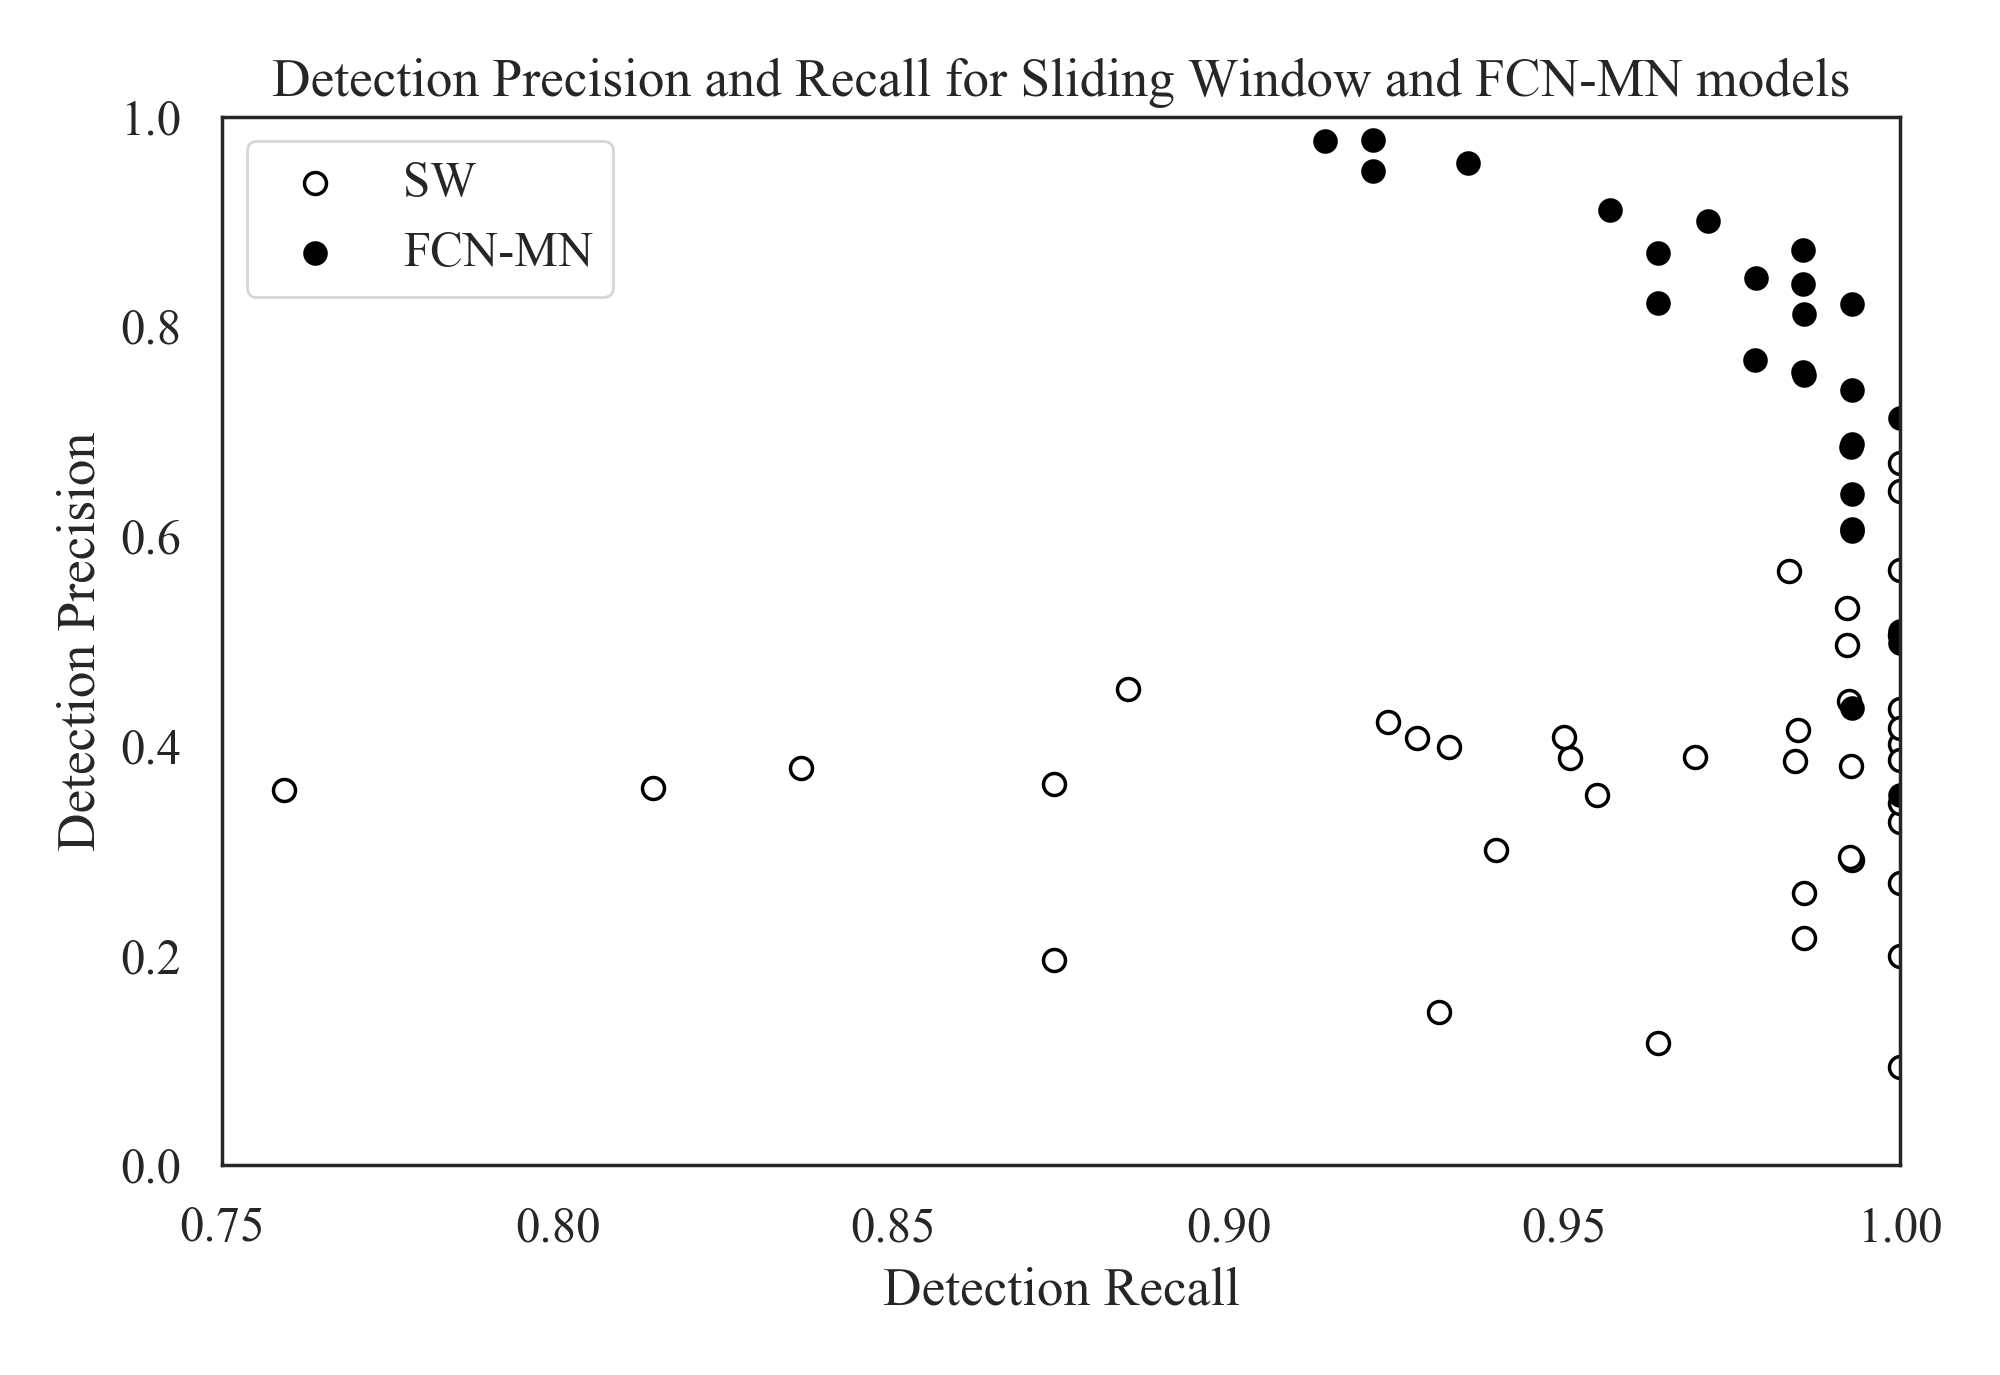
\includegraphics[width=\textwidth]{figures/111_precision_recall_detection.png}
    \caption{
Precision-Recall scatterplots of the second and third columns of Table $\sim$\ref{tab:TablaXX} discriminating the results for FCN-MN and SW with black and white dots, respectively. Each dot then represents the detection-precision and detection-recall computed over all test images, for some particular configurations of hyper-parameters. For FCN-MN, these hyper-parameters would be the architecture, with values 8s, 16s and 32s, and threshold $\tau = \{0.1, 0.2, \ldots, 0.9\}$  for a total of $27$ black dots, while for SW, the hyper-parameters would be the patch sizes  $\{100, 200, \ldots, 1000\}$ and voting thresholds $\{1, 2, 3, 4\}$ for a total of 40 white dots.
    }
    \label{fig:detection-scatter-plot}
\end{figure}


Detection-precision and detection-recall are computed over a combination of correctly detected and splitted components. To easily assess the impact of the split cases, Figure $\sim$\ref{fig:number-of-split} shows the $S$ values corresponding to the fifth column of a   (non-summarized version of) Table $\sim$\ref{tab:TablaXX} in the form of a histogram, with bins representing values of $S$ and the bars for that bin representing the proportion of models that resulted in that value of $S$. Black and white bars discriminate the cases for FCN-MN and SW, respectively. For instance, the first bin indicates that approximately $54\%$ of the FCN-MN models and approximately $62\%$ of the SW models resulted in a total number splits of less than $5$. Overall, the FCN-MN distribution is slightly more concentrated in the lower number of splits than the SW distribution, but in general both algorithms compare fairly, with no clear contender when compared with the average number of splits they produce. 


\begin{figure}
    \centering
    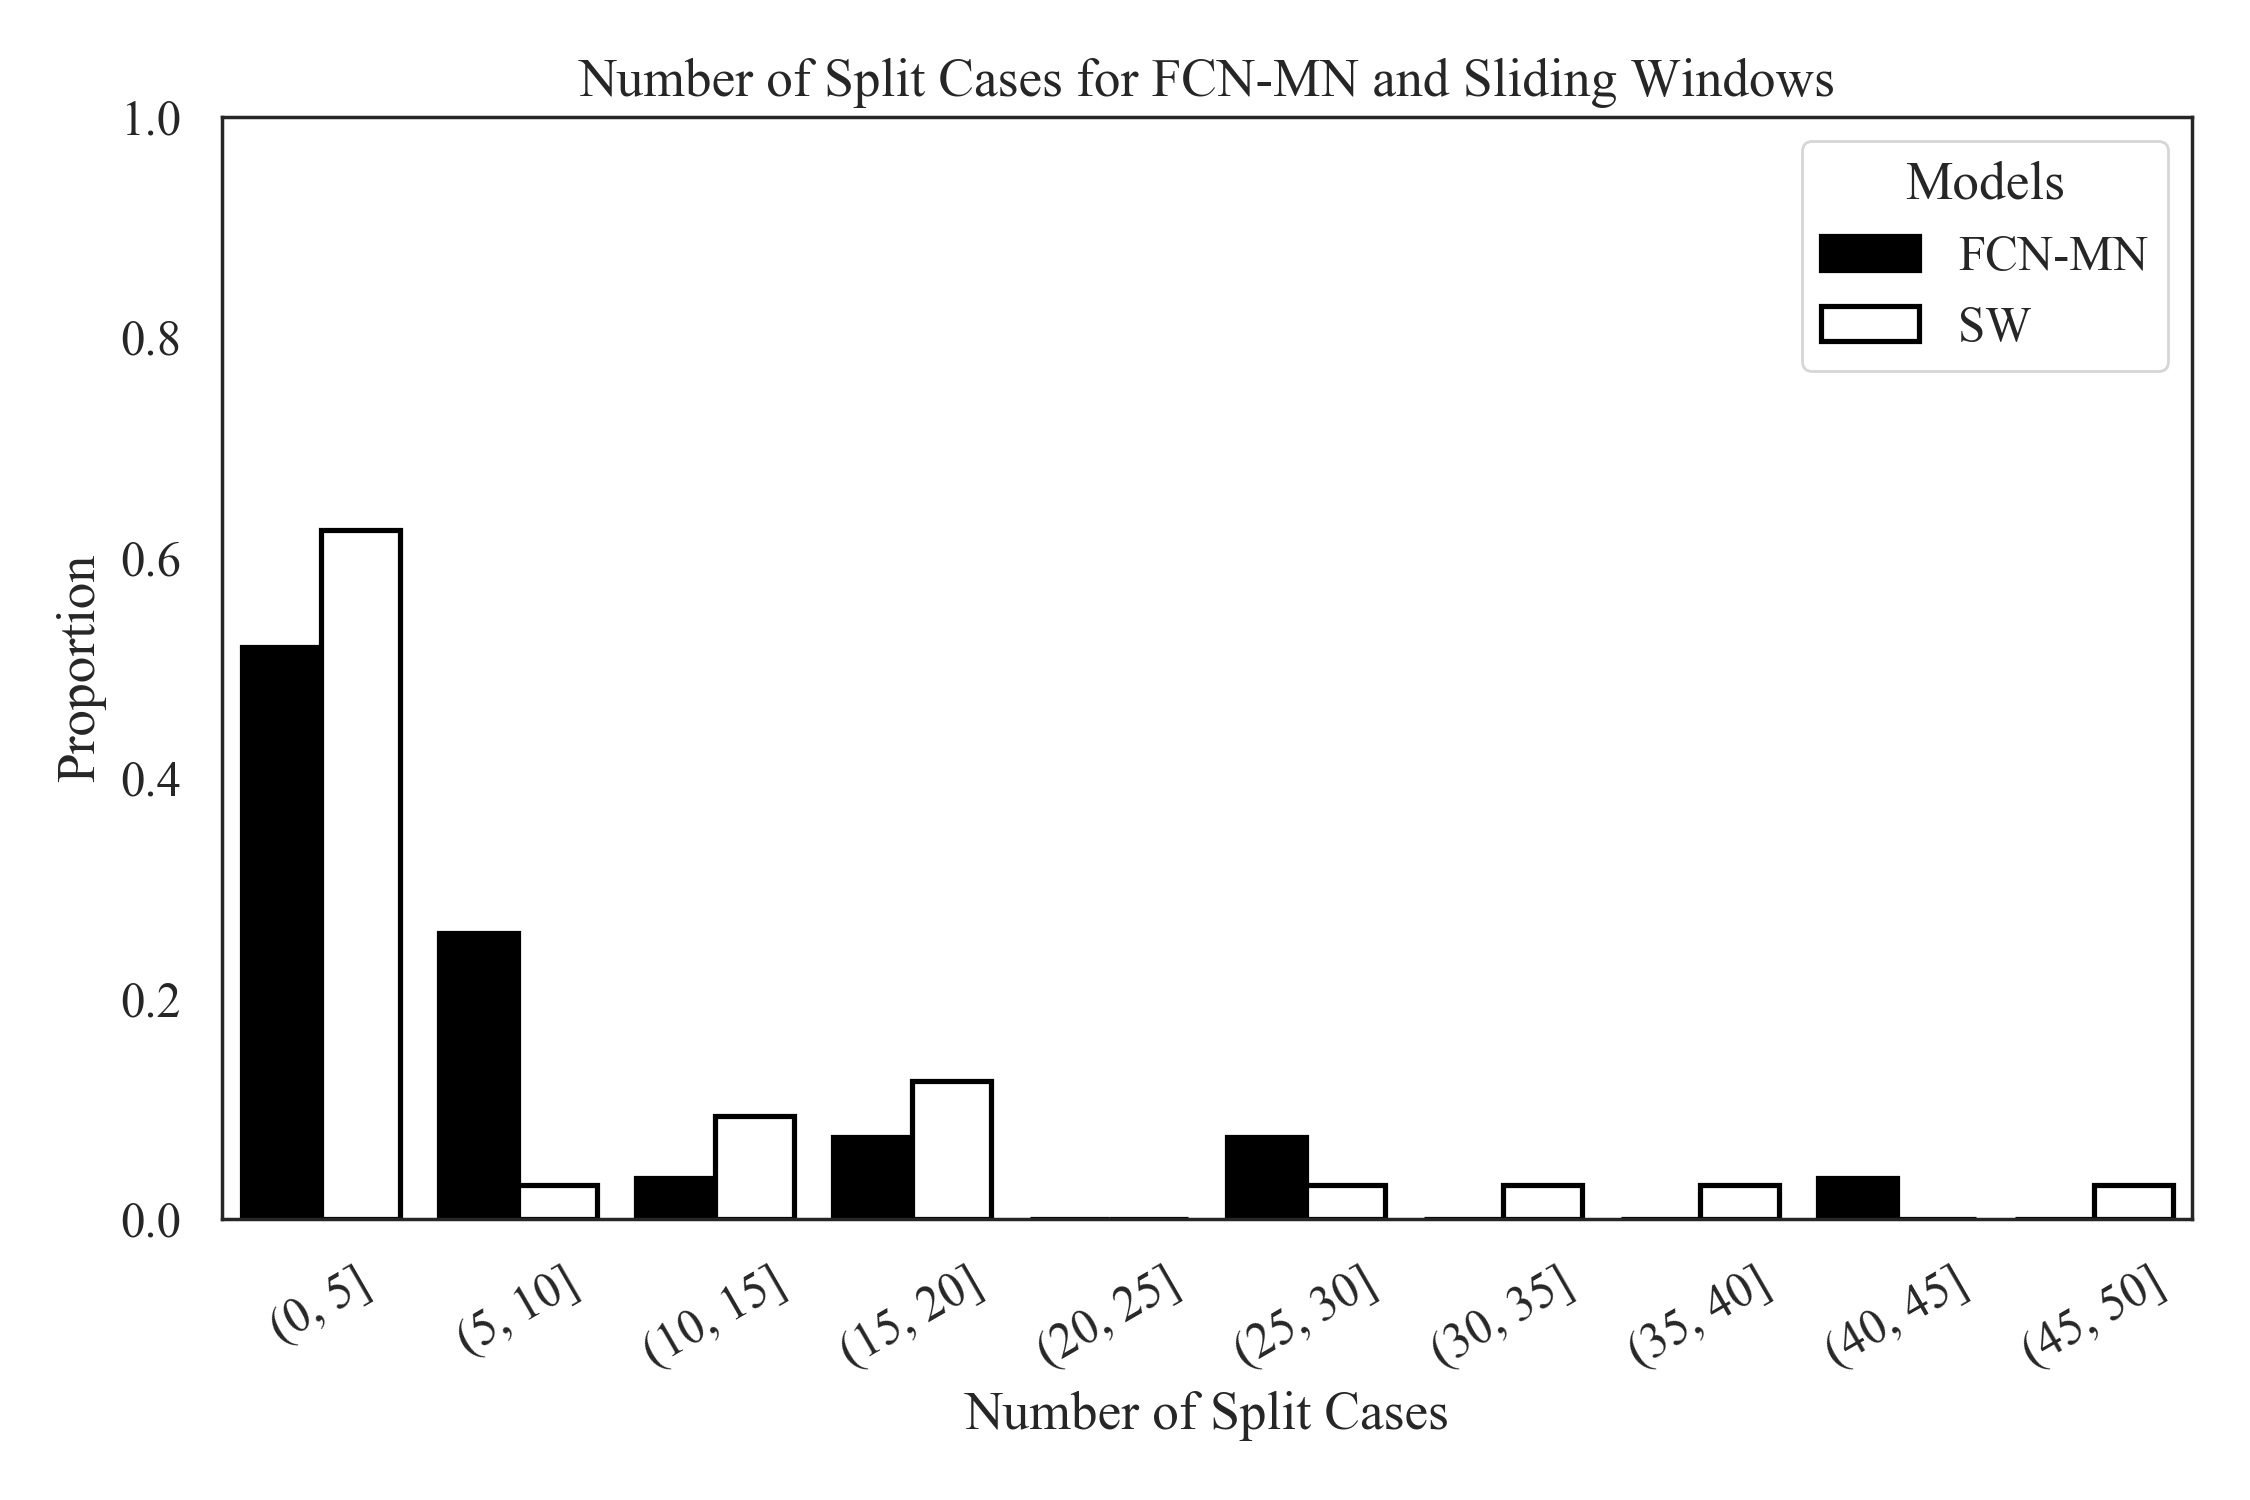
\includegraphics[width=\textwidth]{figures/PPP_split_distribution.png}
    \caption{
Histogram reporting the distribution of $S$ for FCN-MN and SW in black and white bars, respectively. Each bar represents the proportion among all models ($27$ for FCN-MN  and $40$ for SW) that contains the number of splits indicated by the bin label. For instance, the first (from left to right) white bar indicates that almost $14\%$ out of the $40$ SW models contains between $0$ and $5$ splits.
    }
    \label{fig:number-of-split}
\end{figure}


\subsubsection{Detailed analysis of segmentation metrics}

As for the correspondence identification metric, Figures$\sim$ \ref{fig:XXX-a} and \ref{fig:XXX-b} show scatter plots for segmentation-precision and segmentation-recall and for \emph{correct detection} and \emph{split} cases, respectively. These correspond to their respective columns of (a non-summarized version of) Table $\sim$\ref{tab:TablaXX} with black and white dots representing the values of FCN-MN and SW detection models, respectively. The position of each dot in the plot corresponds to the mean segmentation-precision and mean segmentation-recall over all images in the test set, computed over the correctly detected components (splitted components, respectively) of the masks produced by the detection model associated to that dot. The standard deviation of the recall (precision) is shown as a horizontal (vertical) bar.

In Figure $\sim$\ref{fig:XXX-a} (correct detections), one can observe that all black dots (FCN-MN) are clustered in the upper-right corner of the graph, enclosed by a minimum precision of approximately $0.65$ and minimum recall of approximately $0.60$, while the white dots (SW) are clustered in the lower-right corner of the graph with maximum precisions of $0.5$ and recall ranging from approximately $0.35$ to $1.0$. Overall, both algorithms show relatively high recalls, but with FCN-MN reaching much larger precisions. We can point to the coarse detection of the SW method as the main cause for low precision, as this is reduced when extra, false positives are present in the positive mask. 

In Figure $\sim$\ref{fig:XXX-b} (splits), one can observe again the overwhelming improvements of FCN-MN over SW, with all (but one) SW cases presenting precisions under $60\%$, with the outlier showing a precision of nearly  $70\%$ and a similar distribution of recall values.  


%Fig XXX. 

\begin{figure}%
    \centering
    \begin{subfigure}[b]{0.45\textwidth}
        \centering
        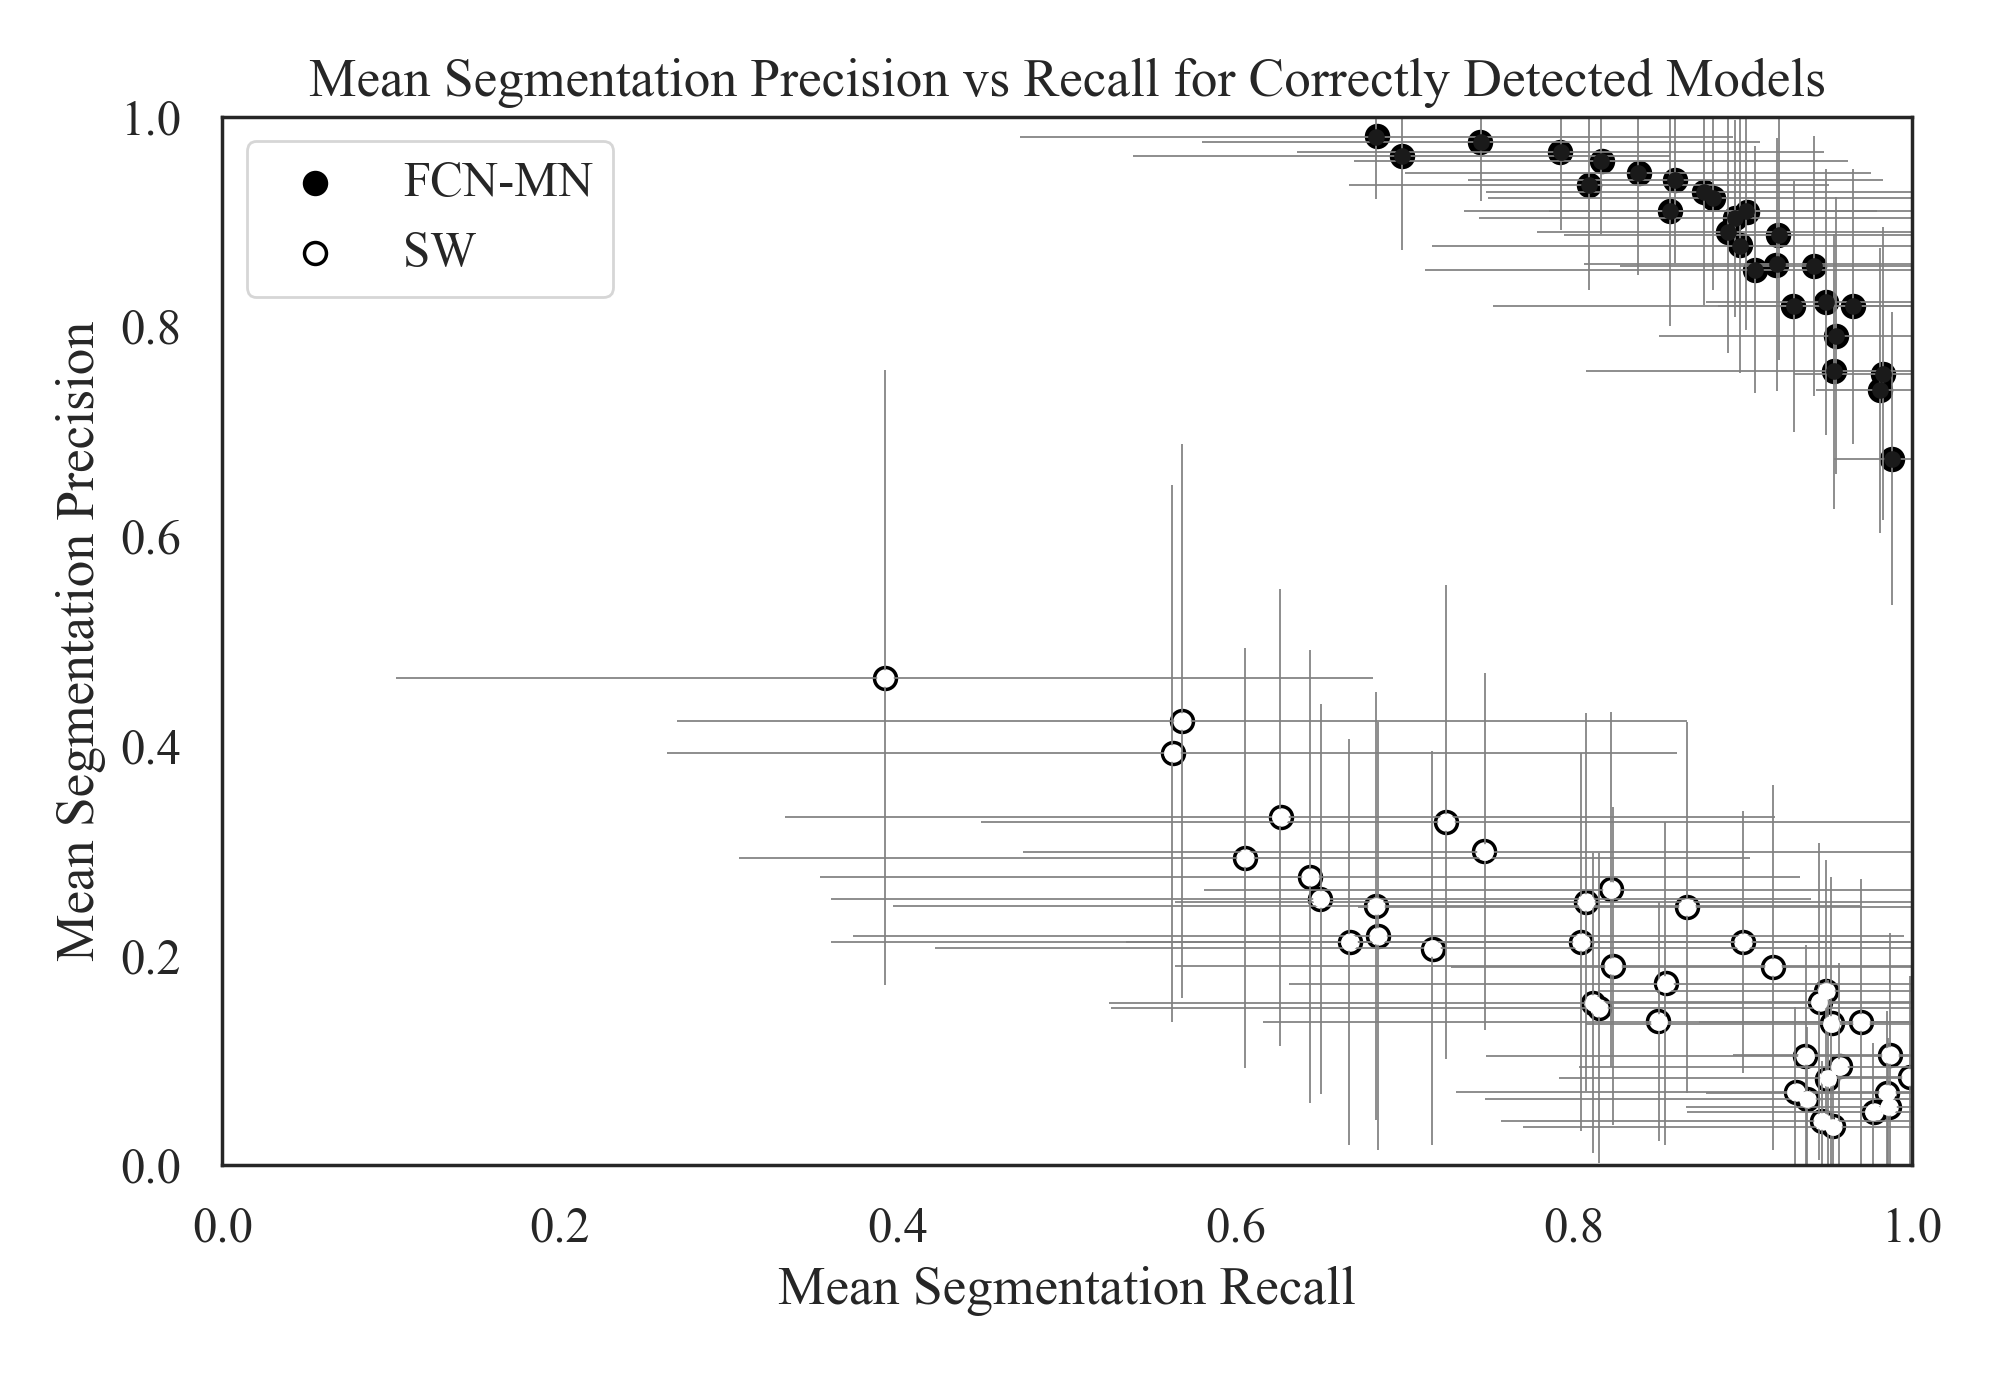
\includegraphics[width=\textwidth]{figures/XXX_correctly_detected.png}
        \caption{}
        \label{fig:XXX-a}
    \end{subfigure}
    \hfill
    \begin{subfigure}[b]{0.45\textwidth}
        \centering
        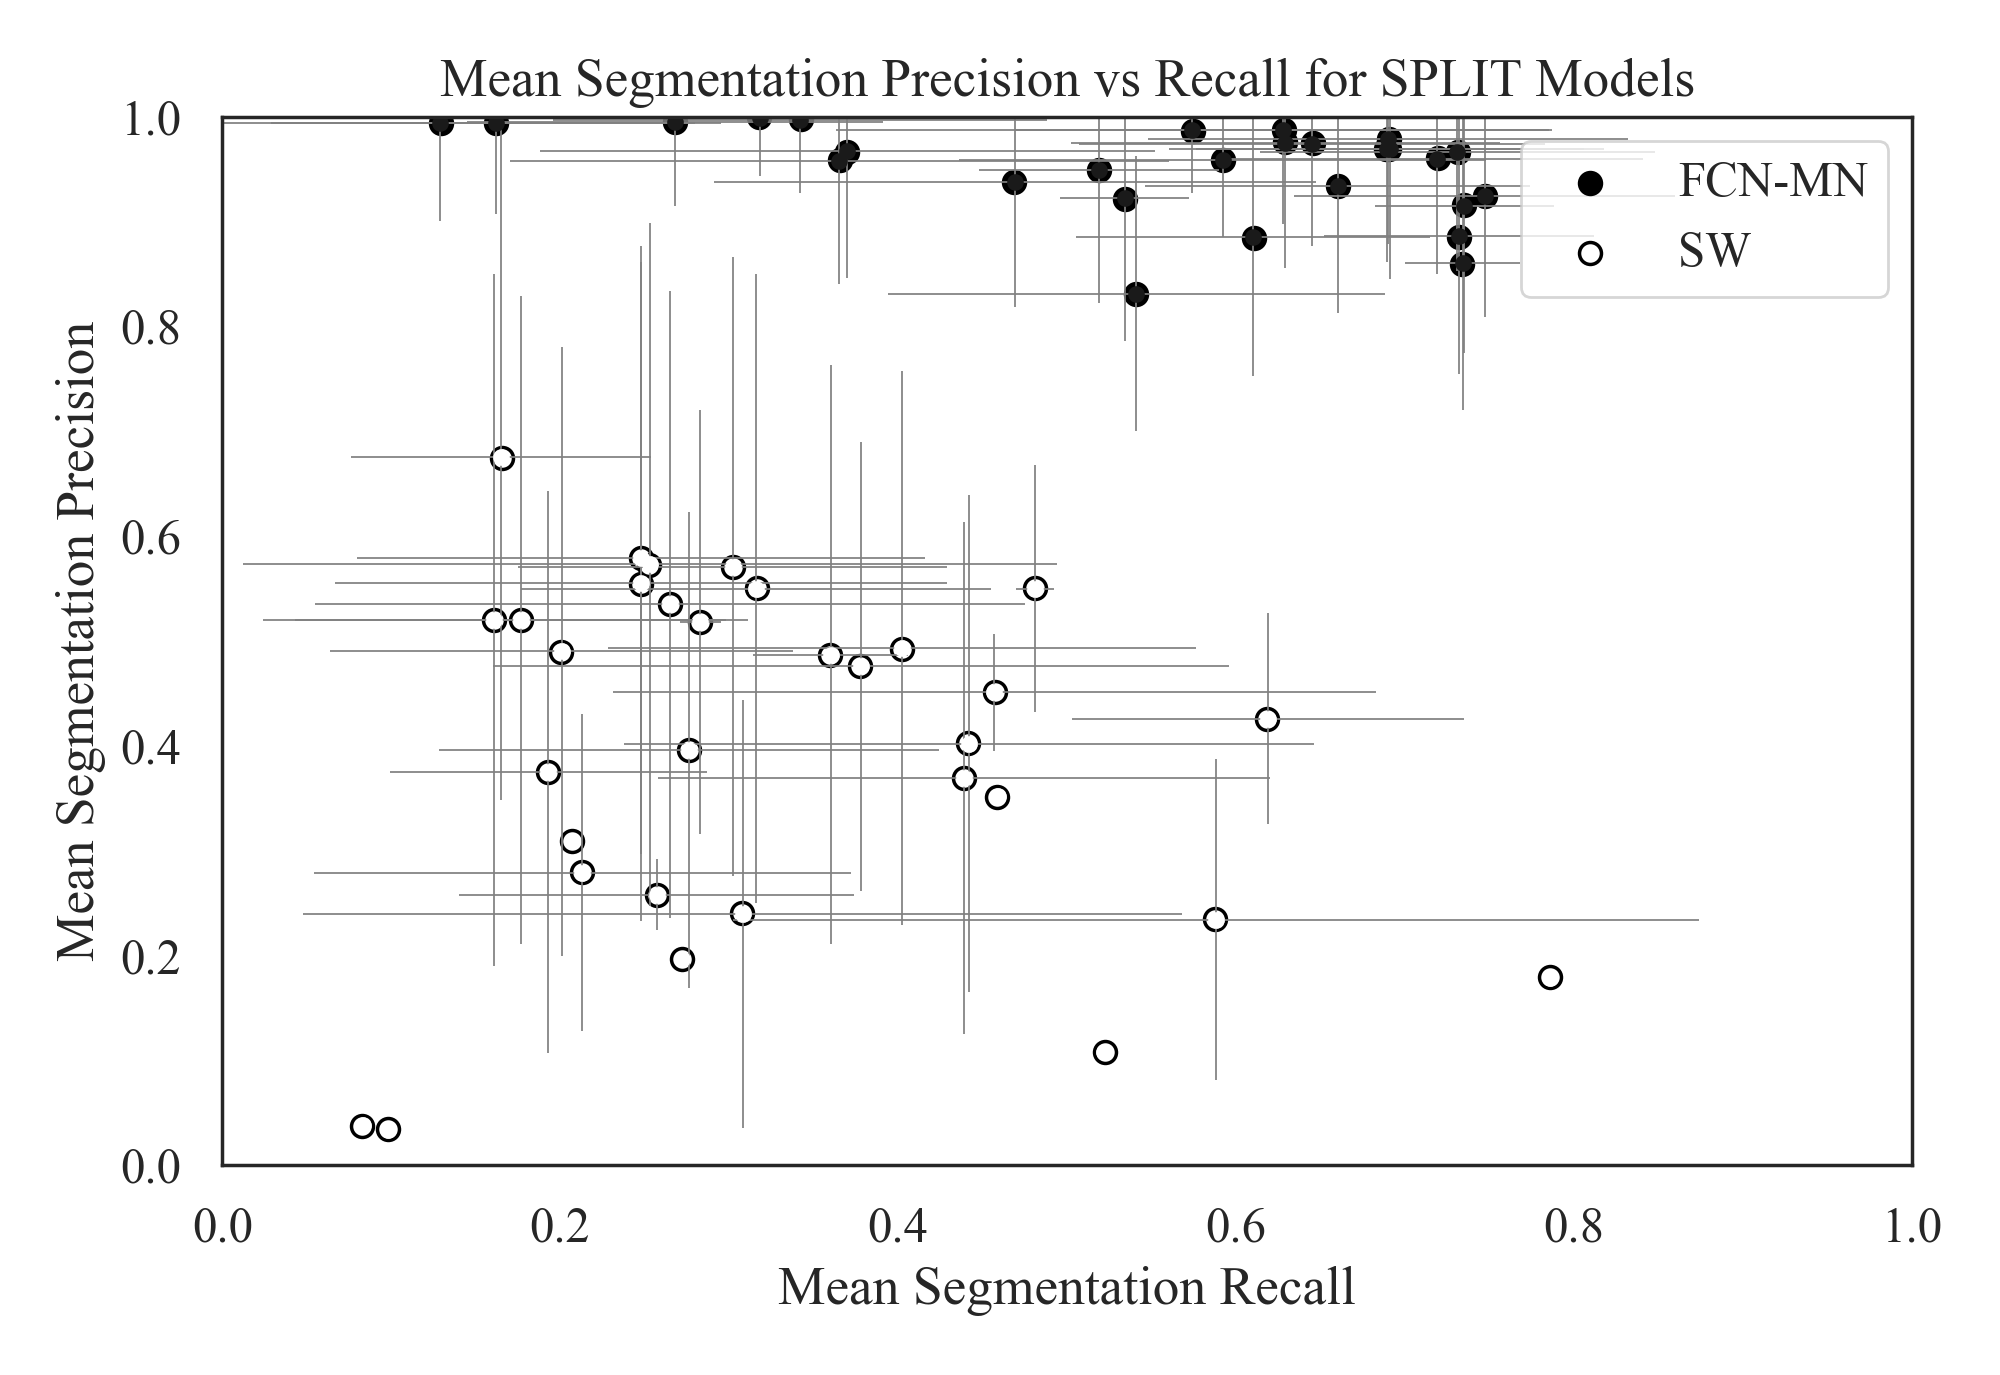
\includegraphics[width=\textwidth]{figures/XXX_splits.png}
        \caption{}
        \label{fig:XXX-b}
    \end{subfigure}
\caption{
Segmentation Precision-Recall scatterplots reporting the results for FCN-MN and SW in black and white, respectively, with dots representing the segmentation precision and segmentation recall average over all images in the test set (and bars representing standard deviations) with one dot per hyper-parameter configuration ($27$ for FCN-MN  and $40$ for SW). In (a) averages were computed over the segmentation precision and recall of correctly detected components, while in (b), averages were computed over the segmentation precision and recall of split components. Standard deviations.
    }%
    \label{fig:XXX}%
\end{figure}








% Figure AAA
\begin{figure}%
    \centering
      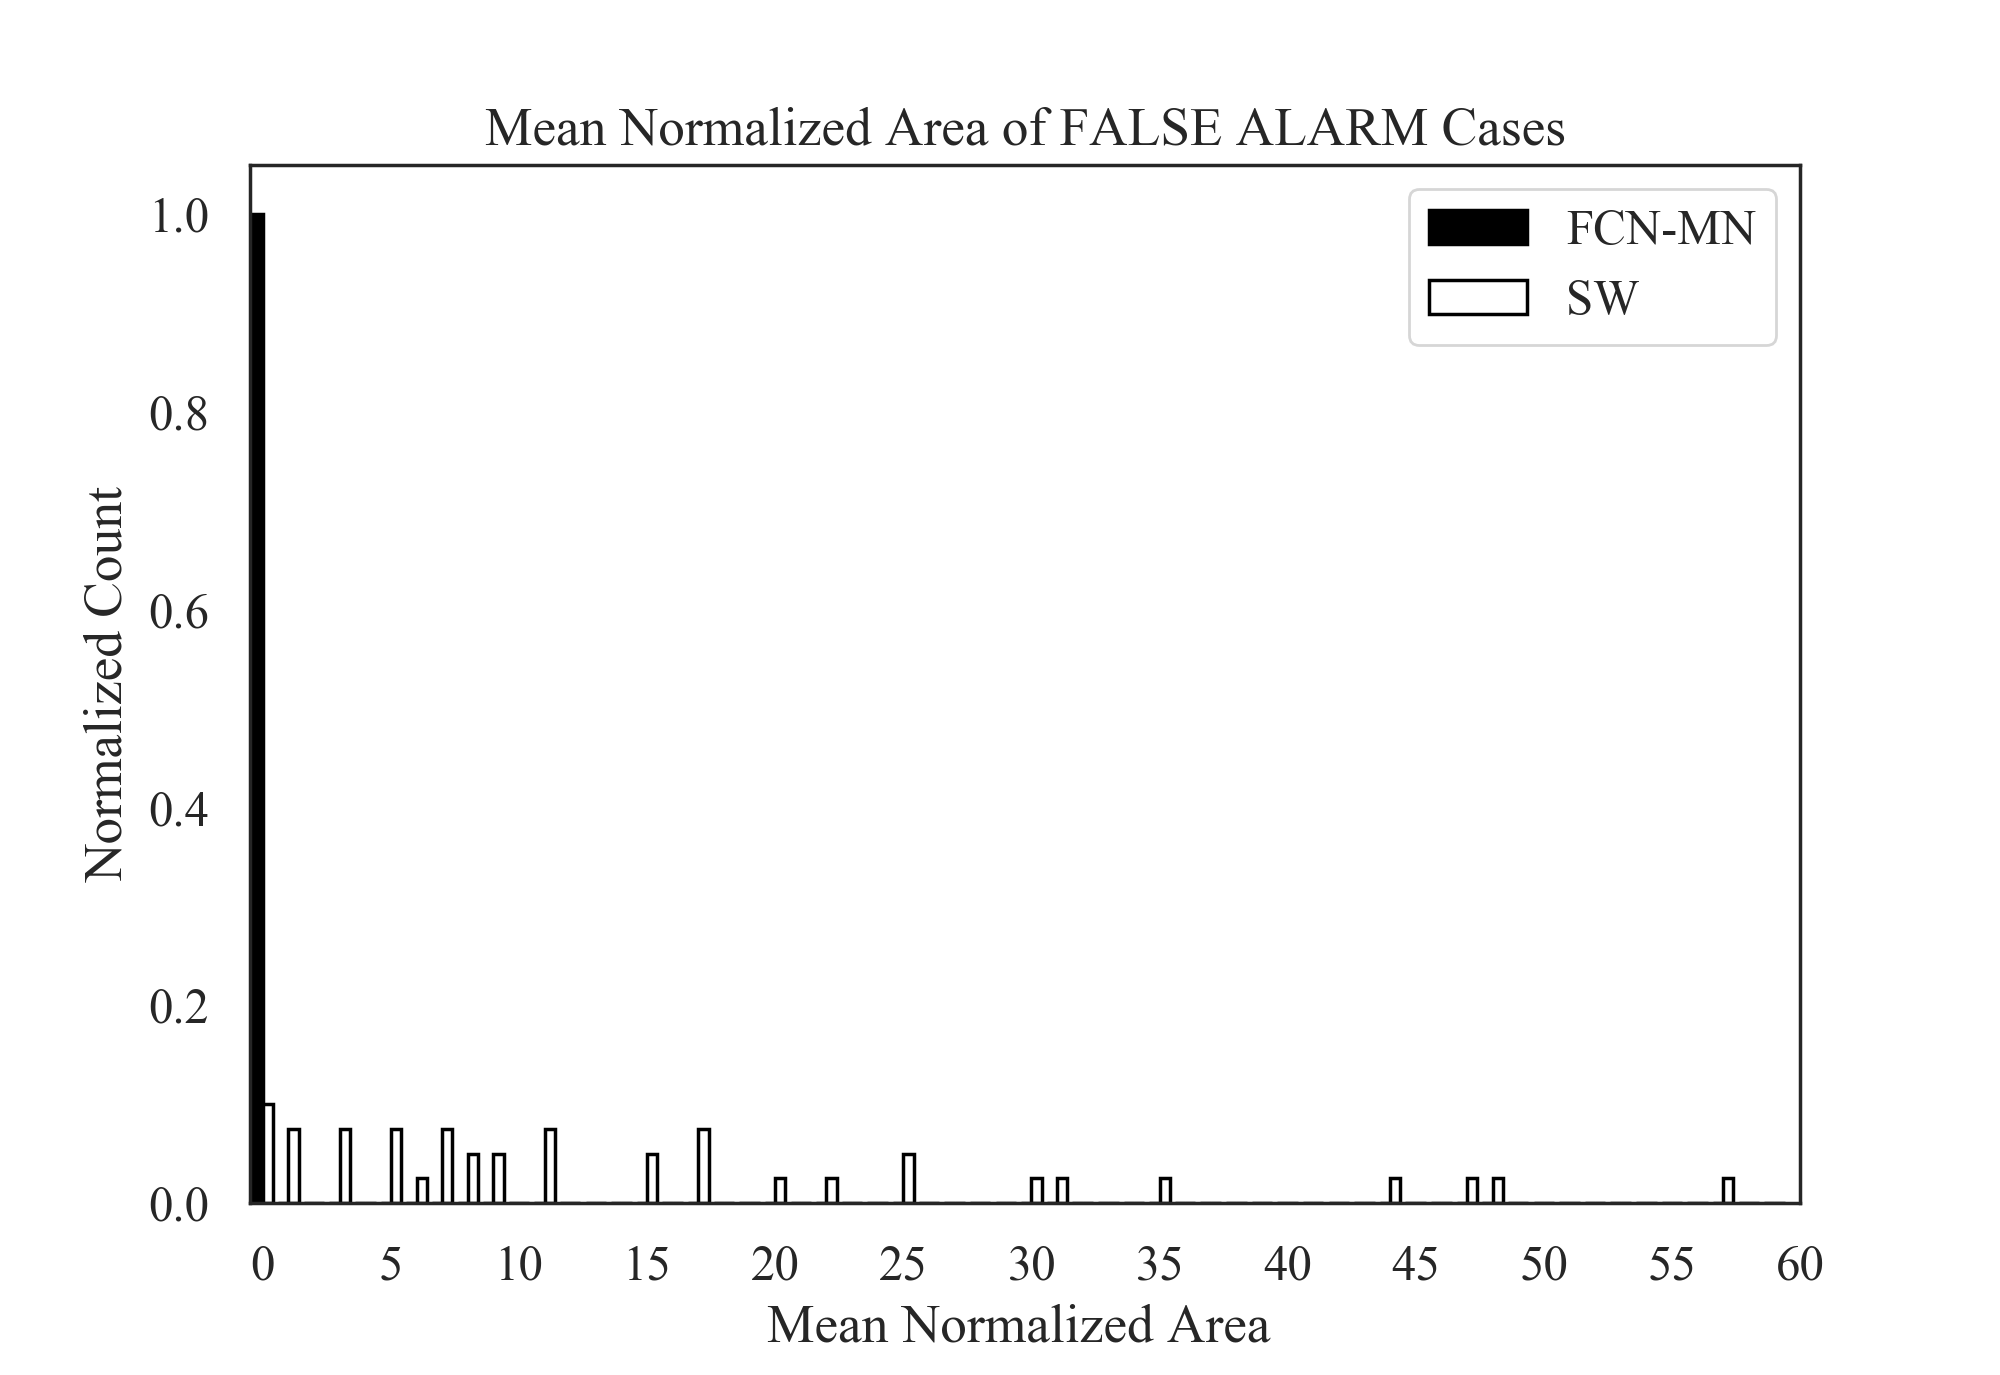
\includegraphics[width=\textwidth]{figures/AAA_mean_relative_area_fcn_vs_sw.png}%
\caption{
FCN-MN (black bars) and SW (white bars) histograms of the mean normalized area $NA$ of false alarm components with bars representing the proportion of detection models whose mean $NA$ falls within the bin interval.
    }
\label{fig:AAA}
\end{figure}


The segmentation results for the false alarm, the $NA$  for each of the $27$ models of FCN-MN and each of the $40$ models of SW, i.e., for each cell in the  one-before-last column of (a non-summarized version of) Table $\sim$\ref{tab:TablaXX} are reported graphically. Figure $\sim$\ref{fig:AAA} shows these results grouped in the form of two histograms, one for the FCN-MN detection models (black) and one for the SW models  (white). Bars in the histogram represent the proportion of detection models whose mean $NA$ (over all false alarm components of all images) falls within the bin interval. The more concentrated to the left the better the algorithm, as this indicates that more detection models for that algorithm resulted in smaller $NA$ (on average).

One can observe the histogram for FCN-MN considerably more concentrated in the left-most part of the histogram than that of SW, with all FCN-MN concentrated in a single bar at the left-most interval of $[0.0, 1.0)$. For SW, the situation is rather different with bars at intervals as far to the right as $[57.0, 58.0)$, that is, detection models with areas as large as $58$ times the bud area. 

\subsubsection{Detailed analysis of localization metrics}

To conclude, this subsection presents a graphical representation of the localization results reported in Table $\sim$\ref{tab:TablaXX}, that is,  the \emph{normalized distance} ($ND$) only for false alarms. This assumes that, because they overlap the true bud, correctly detected and split cases should be close enough to the true bud to render unnecessary any analysis on their distance. Instead, a false alarm can be arbitrarily far from the true bud. 

Figure $\sim$\ref{fig:AAA_ND} summarizes the $ND$ values reported in the corresponding column of the (non-summarized version) of Table $\sim$\ref{tab:TablaXX} in the form of two histograms, one for FCN-MN (black) and one for SW (white).  Bars in the histogram represent the proportion of detection models ($27$ for FCN-MN and $40$ for SW) whose mean $ND$ (over all false alarm components of all images) falls within the bin interval. The more concentrated to the left the better the algorithm, as this indicates that more detection models for that algorithm resulted in smaller $ND$ (on average).

Here again the advantage of FCN-MN over SW is clear, with the histogram for FCN-MN more concentrated in the left-most part than that of SW, with the FCN-MN histogram running from the $(0,1]$ to the $(7,8]$ bin and the SW histogram running from the $(5,6]$ towards the $(9,10]$ bin. 

\begin{figure}%
    \centering
  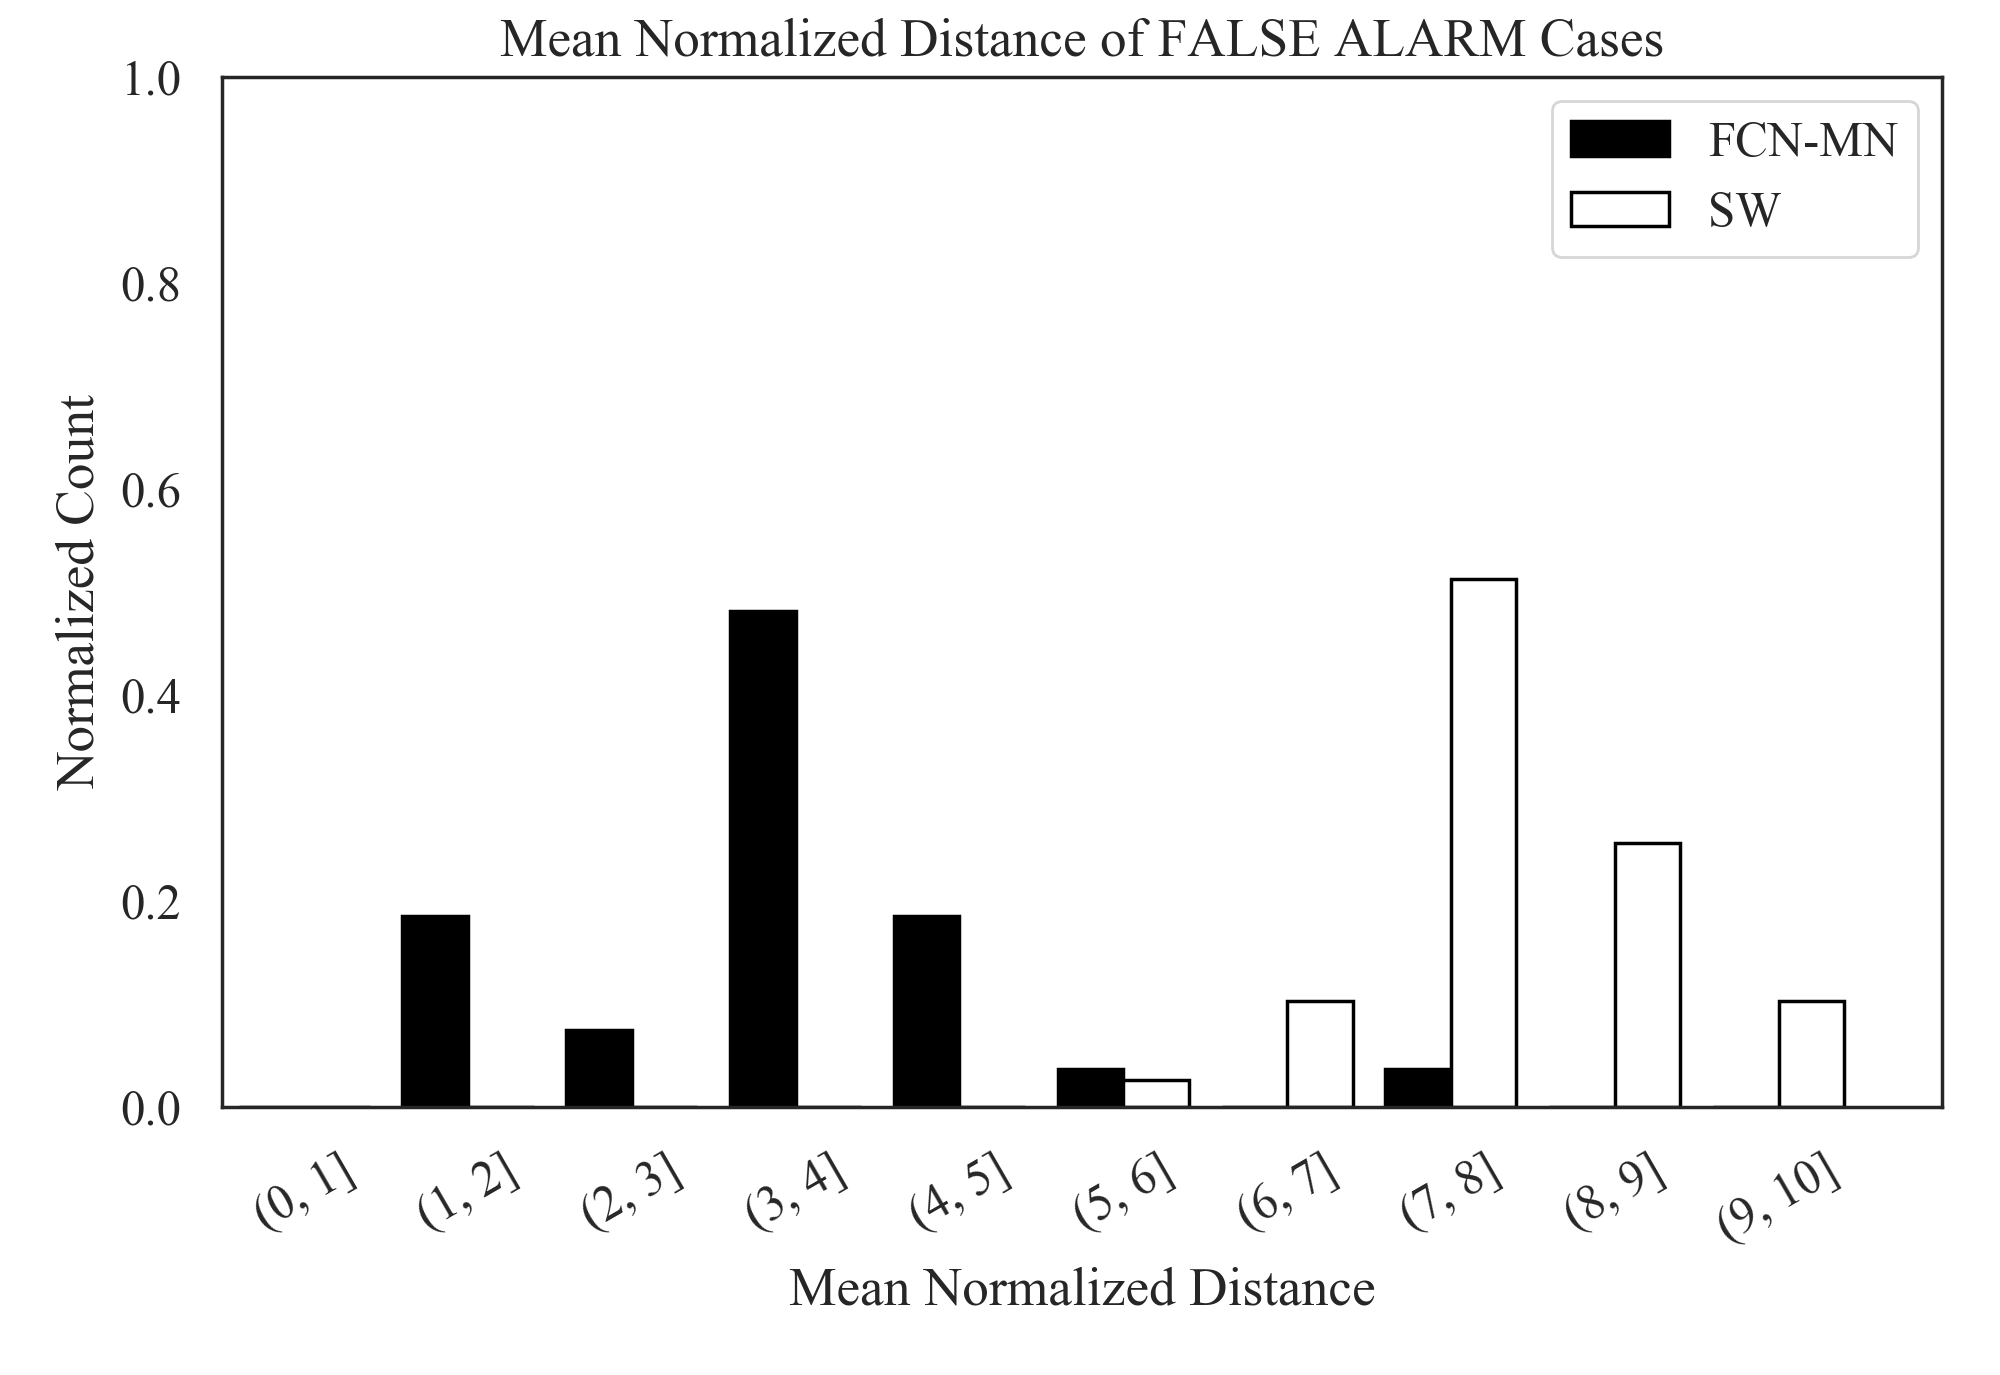
\includegraphics[width=\textwidth]{figures/AAA_normalized_distance_falsealarm_fcn_sw.png}%
\caption{
FCN-MN (black bars) and SW (white bars) histograms of mean normalized distance $ND$ over all false alarm components with bars representing the proportion of detection models whose mean $ND$ falls within the bin interval.
    }
\label{fig:AAA_ND}
\end{figure}


\section{Discussion and Conclusions}
\label{sec:discussion}

This section discusses the results obtained by the proposed approach in the context of the problem of grapevine bud detection and its impact as a tool for measuring viticultural variables of interest. It also highlights the most important conclusions and presents future work. 

This work introduces FCN-MN, a fully convolutional network with Mobile Net architecture for the detection of grapevine buds in 2D images captured in natural field conditions in winter (i.e., no leaves or bunches) and containing a maximum of one bud.

The experimental results confirmed our main hypothesis: that the detection quality achieved by FCN-MN is improved over the \emph{sliding windows} detector (SW) in all three detection aspects: segmentation, correspondence identification and localization. Being SW the best bud detector known to these authors, one can conclude that FCN-MN is a strong contender in the state-of-the-art for bud detectors. However, even improving over these, one can still wonder if it can address the main \emph{quality} requirements of a practical measurement of the bud-related variables in Table $\sim$\ref{tab:Tabla1}.

Quality performance could be assessed by the metrics reported in Table $\sim$\ref{tab:TablaXX}. In the best case, FCN-MN shows a  detection-precision and detection-recall of $97.7$ and $100$, respectively, a mean (and standard deviation) segmentation-precision and segmentation-recall for correct detections of $98.1(0.6)$ and $98.8(3.4)$, respectively, and for splits $99.9(0.1)$ and $74.7(28.1)$, respectively. For false alarms, it shows a maximum  $NA$ of $0.04(0.09)$ and a maximum $ND$ of $0.04 (0.22)$.  

However, each of these maximums correspond to different FCN-MN detectors. A better assessment must be conducted for a single detector. For that, we picked FCN-MN$_{16s}^{0.6}$ to show balanced quality overall. This detector reaches detection precision and recall of $95.6$ and $93.6$, respectively, meaning than only $4.4\%$ of all the detected connected components over all test images are false alarms, and that only $6.4\%$ of all true buds could not be detected (i.e., resulted in detection failure).

Additionally, $S=3$, meaning only $3$ of all detections were splitted, which has a segmentation precision of $99.4(0.6)$ and a segmentation recall of $16.2(10.6)$ on average. The recall is rather small, suggesting that the split is, in fact, the result of pixel-wise detection of the bud so sparse that it became disconnected. In contrast, all remaining detections were correct (i.e., not splitted), reaching segmentation precisions of $92.2(8.7)$, a rather similar value to that of splits, but a much larger mean segmentation recall of $88.2(13.3)$. Overall, this resulted in a mean Dice measure for the correct detections of $89.1(10.7)$, demonstrating a considerable (mean) coverage of the true bud with only $11.8\%$ of the bud pixels missing (on average) and only $7.8\%$ of the detected pixels covering the background (on average).

More promising, however, are the false alarm results with $NA=0.08$ and $ND=1.1$, showing that these components are rather small covering only an area that is $8\%$ in size of the total bud area (on average) and distant to the true bud by only $1.1 (0.65)$ diameters.

Based on these results, what quality should one expect when the FCN-MN$_{16s}^{0.6}$ detector takes part in the measurement of the bud-related variables? For brevity, this point is discussed for three variables from Table $\sim$\ref{tab:Tabla1}: \emph{bud number}, \emph{bud area}, and \emph{internode length}.

The case of \emph{bud number}, for example, requires identifying correspondences for buds in the scene, so its quality will be impacted only by the metrics of detection precision and recall ($95.6$ and $93.6$, respectively). To evaluate this impact, we assume that a plant has approximately 240 buds on average. The number of buds per plant depends on many factors, such as training system, grape variety, type of treatment, time of year, among others, so this value is defined as indicative to achieve an approximate analysis. For this case, a detection precision of $95.6$ would result in 11 buds counted in excess per plant, while a recall of $93.6$ would result in the omission of 15 buds in the count. 

In addition, this model produces 3 splits with two components each, i.e. a counting error in excess of $3\%$ over the 140 buds in the test set. Particularly in this analysis, it means that $6$ new buds would be counted in excess, giving a total of $17$ buds in excess, practically cancelling out with the error of omission. But additionally, these errors could in practice be statistically characterized allowing for measurement correction towards more accurate values. Despite these good results, our approach still has practical limitations for the measurement of bud number due to the impossibility of automatically associating counts of the same bud in two different images, making it difficult to massively measure the bud count of a plant or plot. 

The second variable of interest considered is \emph{bud area}, where, in addition to identifying correspondences for the buds of a scene, it is necessary to segment it to estimate its area in pixels. Correspondence identification analysis is analogous to bud counting, so now only segmentation metrics are discussed. From the analysis developed in the previous paragraphs, it can be concluded that the segmentation errors by splits and false alarms have a low impact in the general results and, therefore, in the estimation of \emph{bud area}. On the other hand, if we compensate the segmentation errors for the correct detections (i.e. $11.8\%$ of the bud pixels missing and $7.8\%$ of the detected pixels covering the background), the area estimation error is only $4\%$. For illustrative purposes, we see that this error is smaller than the precision error resulting from measuring the area of a bud with a caliper. If we assume that the shape of a bud fits a circle, and that the typical diameter of a bud is $5$ mm, the resulting area is $19.63 mm^2$. Since a caliper has an accuracy of $0.1 mm$, the area precision error would be $\pm 1.7 mm^2$, equivalent to $8.6\%$ of the total area, a figure that doubles the $4\%$ error produced by our FCN-MN detector. To this difference,  the error of manual measurement resulting from assuming a circular bud shape must be added, an unnecessary approximation in the case of FCN-MN.

As in the case of counting, these good results in measurement precision are limited to achieve a practical use of this type of measurement because it is impossible to automatically associate area measurements of the same bud in two different images, making it difficult to systematically measure this variable for the buds of a plant or plot. Furthermore, in this case, the areas obtained are in pixels, which need to be converted into length or area magnitudes.

Finally, let us consider the case of \emph{internode length}, estimated by the distance between buds of the same branch (by the closeness between buds and nodes), which involves the operations of correspondence identification and localization. Again, correspondence identification analysis is analogous to bud counting, which in this case will result in the reporting of more than one distance due to the detection of more than one component per bud. Among these distances, we understand that the worst case can occur between false alarms -these being the farthest from the true bud- and between two buds when the false alarms are at a distance of $ND$ from the farthest side of the other bud. On average, it is $ND = 1.1$, which according to the typical diameter of vine buds is equivalent to about $5$mm, a value much lower than the typical bud distances of approximately $15$cm, i.e., about a $6.6\%$ error in estimating the distance between buds/nodes. 

A limitation of our approach to achieving practical use of this type of measurement is the possibility of determining when two buds are on the same branch, which requires knowledge of the plant structure. Furthermore, with our method, only the distance projected in the image plane could be measured, which can arbitrarily differ from the actual distance in 3D. The  greatest impact errors occur because of the excess or omission of connected components, with the excess error exacerbated by the fact of associating detected buds with individual connected components. A possible improvement to mitigate these errors would be to apply some post-processing. 

One such post-processing is \emph{spatial clustering} of connected components grouping them by proximity. One could expect this to improve the results based on the small areas of split and false alarm components. First, due to the closeness of the false alarms to the true bud  (small $ND$) -as well as the splits and correctly detected components (overlapping with it)-,  and the fact that true buds in real plants are typically tens or even hundreds of bud diameters apart, a simple spatial clustering of the components would connect all of them together as a single, and correct, bud detection. Second, due to their small area -if clustered together- the false alarm components would only slightly reduce segmentation precision.

Another possible post-processing would be to rule out small connected components, for example, whose area in pixels normalized to the total detected area (sum of the areas of all connected components) is less than a certain threshold. Improvements could be expected with this post-processing, since the results in this work show that false alarms present small areas in relation to the true bud. Lastly, connected component filters could be considered based on plant structure, for example, ruling out connected components that are far away from (or do not overlap with) branches.

One could also consider in future works some improvements to overcome the limitations for practical use mentioned above: (i) no associations between plant parts of different images, (ii) distance and area measurements in pixels, (iii) only 2D geometry, (iv) lack of knowledge of underlying plant structure, and (v) need of images with no leaves. 

One could also extend to buds the work of \citet{santos2020grape} that addresses limitation (i) for grape bunches. Limitation (ii) could be easily addressed by adding to the visual scene some marker with known dimensions. This, however, requires such a marker in every image captured, a problem that could be overcome by first producing a calibrated 3D reconstruction of the scene, i.e., a 3D reconstruction calibrated with a single marker in one of its frames \citep{hartley2003multiple, moons20093d}. In this way, every 2D image could be calibrated against the 3D model, omitting the need for a marker. In addition, a 3D reconstruction of the scene could address limitation (iii) by locating the detected buds in 3D space, following, for instance, the approach taken by \citet{diaz2018grapevine}. Finally, a solution to limitations (iv) and (v) would require an integrated approach involving the detection in 3D of branches and leaves, respectively. 

\section*{Acknowledgments}

This work was funded by the National Technological University (UTN), the National Council of Scientific and Technical Research (CONICET), Argentina, and the National Fund for Scientific and Technological Promotion (FONCyT), Argentina.

%\section*{References}
\bibliography{2020-DeepBudDetection-CEA}

\end{document}



